\pdfoutput=1
% TSCG: Token-Context Semantic Grammar for Causal Prompt Optimization in LLMs
% ============================================================================
% To compile: pdflatex main && bibtex main && pdflatex main && pdflatex main
%
% Required style files (download from https://github.com/acl-org/acl-style-files):
%   - acl.sty
%   - acl_natbib.bst
% Place both in this directory before compiling.
% ============================================================================

\documentclass[11pt,a4paper]{article}
\usepackage{acl}
\usepackage{times}
\usepackage{latexsym}
\usepackage{amsmath}
\usepackage{amssymb}
\usepackage{amsfonts}
\usepackage{graphicx}
\usepackage{booktabs}
\usepackage{multirow}
\usepackage{array}
\usepackage{tikz}
\usetikzlibrary{arrows.meta,positioning,shapes.geometric,fit,calc,patterns,decorations.pathreplacing}
\usepackage{pgfplots}
\pgfplotsset{compat=1.18}
% xcolor already loaded by acl.sty
\usepackage{enumitem}
\usepackage{subcaption}
\usepackage{algorithmic}
\usepackage{algorithm}
\usepackage{cleveref}
\usepackage{microtype}
\usepackage{tabularx}
\usepackage{makecell}
\usepackage{pifont}
\usepackage{amsthm}

% Theorem-like environments
\newtheorem{definition}{Definition}[section]
\newtheorem{theorem}{Theorem}[section]
\newtheorem{corollary}{Corollary}[section]
\newtheorem{proposition}{Proposition}[section]
\newtheorem{hypothesis}{Hypothesis}[section]

% Check and cross marks for tables
\newcommand{\cmark}{\ding{51}}
\newcommand{\xmark}{\ding{55}}

% Custom colors
\definecolor{tscgblue}{RGB}{41,98,168}
\definecolor{tscggreen}{RGB}{56,142,60}
\definecolor{tscgred}{RGB}{183,28,28}
\definecolor{tscgorange}{RGB}{230,126,34}
\definecolor{tscggray}{RGB}{117,117,117}
\definecolor{tscgpurple}{RGB}{128,0,128}
\definecolor{tscgteal}{RGB}{0,128,128}

% Custom commands
\newcommand{\tscg}{\textsc{Tscg}}
\newcommand{\principle}[1]{\textsc{#1}}
\newcommand{\fragility}{\mathcal{F}}
\newcommand{\density}{\mathcal{D}}
\newcommand{\attn}{\mathrm{Attn}}
\newcommand{\pos}{\mathrm{pos}}
\newcommand{\tok}{\mathrm{tok}}
\newcommand{\sem}{\mathrm{sem}}
\newcommand{\placeholder}[1]{\textcolor{tscgorange}{#1}}

\title{TSCG: Token-Context Semantic Grammar for Causal Prompt Optimization\\in Large Language Models}

\author{Furkan Sakizli \\
  Independent Researcher \\
  \texttt{furkan.sakizli@gmail.com}}

\begin{document}
\maketitle

% =============================================================================
% TAB Benchmark Paper Tables (Plan 5.1)
% Auto-generated from benchmark results: 2026-03-03
% =============================================================================

% -----------------------------------------------------------------------------
% Table 1: Frontier Model Results (Scenarios A + B)
% Data: benchmark/results/frontier/a/ and b/
% Data: benchmark/results/frontier-natural-text/a/ and b/
% -----------------------------------------------------------------------------

\begin{table*}[t]
\centering
\small
\begin{tabular}{@{}ll cccc cc@{}}
\toprule
& & \multicolumn{4}{c}{\textbf{Accuracy (\%)}} & \multicolumn{2}{c}{\textbf{Savings}} \\
\cmidrule(lr){3-6} \cmidrule(lr){7-8}
\textbf{Model} & \textbf{Condition} & \textbf{Sc.~A} & \textbf{95\% CI} & \textbf{Sc.~B} & \textbf{95\% CI} & \textbf{Tokens} & \textbf{ARR} \\
\midrule
\multirow{4}{*}{Claude Sonnet 4}
    & Natural (FC)    & 74.0 & [64.6, 85.6] & 90.0 & [86.1, 92.9] & ---   & --- \\
    & Natural (text)  & 51.1 & [42.5, 66.9] & 70.0 & [64.6, 74.9] & ---   & --- \\
    & TSCG            & \textbf{85.2} & [81.9, 96.4] & \textbf{95.0} & [91.9, 96.9] & 50.1\% & 1.15 \\
    & TSCG+SAD        & 76.7 & [70.1, 89.4] & 95.0 & [91.9, 96.9] & 49.5\% & 1.04 \\
\midrule
\multirow{4}{*}{GPT-4o}
    & Natural (FC)    & 55.5 & [44.1, 68.4] & 70.0 & [64.6, 74.9] & ---   & --- \\
    & Natural (text)  & 45.7 & [34.6, 59.1] & 55.0 & [49.3, 60.5] & ---   & --- \\
    & TSCG            & 56.5 & [45.7, 69.9] & \textbf{79.7} & [75.1, 84.1] & 6.2\% & 1.02 \\
    & TSCG+SAD        & 53.2 & [42.5, 66.9] & 81.4 & [76.9, 85.6] & 5.3\% & 0.96 \\
\midrule
\multirow{4}{*}{GPT-5.2}
    & Natural (FC)    & 51.9 & [45.7, 69.9] & 82.4 & [78.7, 87.1] & ---   & --- \\
    & Natural (text)  & 78.3 & [75.8, 93.1] & \textbf{98.2} & [98.7, 100.0] & ---   & --- \\
    & TSCG            & \textbf{81.6} & [79.9, 95.3] & 91.6 & [91.9, 96.9] & 11.4\% & 1.57 \\
    & TSCG+SAD        & \textbf{85.9} & [88.6, 99.1] & 90.9 & [89.9, 95.6] & 10.5\% & 1.65 \\
\bottomrule
\end{tabular}
\caption{TAB Benchmark: Frontier model results on Scenario~A (20 tasks, small catalog) and Scenario~B (100 tasks, large catalog). Each condition evaluated with 3 runs ($n=60$ per cell for Sc.~A, $n=300$ for Sc.~B). \emph{Natural~(FC)} uses the provider's native function calling API; \emph{Natural~(text)} embeds full JSON schemas as text; \emph{TSCG} uses balanced compression as text; \emph{TSCG+SAD} adds aggressive compression with Selective Anchor Duplication. Token savings are relative to Natural~(FC). ARR = Accuracy Retention Rate (TSCG accuracy / Natural~FC accuracy; values $>1.0$ indicate TSCG outperforms the baseline). \textbf{Bold} marks best accuracy per model per scenario.}
\label{tab:tab-frontier}
\end{table*}

% -----------------------------------------------------------------------------
% Table 2: Format vs Compression Effect Decomposition (Wave 2.12b)
% Data: frontier-natural-text vs frontier
% -----------------------------------------------------------------------------

\begin{table}[t]
\centering
\small
\begin{tabular}{@{}l rr rr@{}}
\toprule
& \multicolumn{2}{c}{\textbf{Format Effect}} & \multicolumn{2}{c}{\textbf{Compression Effect}} \\
\cmidrule(lr){2-3} \cmidrule(lr){4-5}
\textbf{Model} & \textbf{Sc.~A} & \textbf{Sc.~B} & \textbf{Sc.~A} & \textbf{Sc.~B} \\
\midrule
Claude Sonnet 4  & $-$22.9 & $-$20.0 & $+$34.1 & $+$25.0 \\
GPT-4o           & $-$9.8  & $-$15.0 & $+$10.8 & $+$24.7 \\
GPT-5.2          & $+$26.4 & $+$15.8 & $+$3.3  & $-$6.6  \\
\bottomrule
\end{tabular}
\caption{Decomposition of the TSCG advantage into format and compression effects (percentage points). \emph{Format effect} = Natural~(text) $-$ Natural~(FC): positive values indicate text-mode is better than native function calling. \emph{Compression effect} = TSCG $-$ Natural~(text): positive values indicate compression improves accuracy beyond uncompressed text. For Claude and GPT-4o, compression is the dominant driver (overcoming a negative format penalty). For GPT-5.2, the text format itself provides the main benefit.}
\label{tab:format-decomposition}
\end{table}

% -----------------------------------------------------------------------------
% Table 3: Small Model Scaling (Scenario D)
% Data: benchmark/results/small-models/
% -----------------------------------------------------------------------------

\begin{table*}[t]
\centering
\small
\begin{tabular}{@{}l c ccc ccc@{}}
\toprule
& & \multicolumn{3}{c}{\textbf{Accuracy (\%)}} & \multicolumn{3}{c}{\textbf{$\Delta$ vs Natural (pp)}} \\
\cmidrule(lr){3-5} \cmidrule(lr){6-8}
\textbf{Model} & \textbf{Tools} & \textbf{Natural} & \textbf{TSCG\textsubscript{cons}} & \textbf{TSCG\textsubscript{bal}} & \textbf{TSCG\textsubscript{cons}} & \textbf{TSCG\textsubscript{bal}} & \textbf{cons $-$ bal} \\
\midrule
\multirow{3}{*}{Mistral 7B}
    & 10  & 83.5 & 76.0 & 73.3 & $-$7.5  & $-$10.2 & $+$2.7 \\
    & 20  & 35.0 & 80.0 & 80.1 & $+$45.0 & $+$45.1 & $-$0.1 \\
    & 50  & 30.0 & \textbf{75.3} & 65.0 & $+$45.3 & $+$35.0 & $+$10.3 \\
\midrule
\multirow{3}{*}{Gemma 3 4B}
    & 10  & 69.1 & \textbf{80.7} & 74.7 & $+$11.6 & $+$5.6 & $+$6.0 \\
    & 20  & 49.9 & \textbf{87.3} & 67.0 & $+$37.4 & $+$17.1 & $+$20.3 \\
    & 50  & 24.3 & 87.5 & \textbf{87.4} & $+$63.2 & $+$63.1 & $+$0.1 \\
\midrule
\multirow{3}{*}{Gemma 3 12B}
    & 10  & 90.0 & --- & \textbf{93.0} & --- & $+$3.0 & --- \\
    & 20  & 85.0 & --- & \textbf{95.0} & --- & $+$10.0 & --- \\
    & 50  & 85.0 & --- & \textbf{98.0} & --- & $+$13.0 & --- \\
\midrule
\multirow{3}{*}{Qwen3 14B}
    & 10  & 94.9 & \textbf{98.8} & 86.2 & $+$3.9  & $-$8.7  & $+$12.6 \\
    & 20  & 90.2 & \textbf{99.3} & 84.1 & $+$9.1  & $-$6.1  & $+$15.2 \\
    & 50  & 94.6 & \textbf{95.0} & 89.6 & $+$0.4  & $-$5.0  & $+$5.4 \\
\bottomrule
\end{tabular}
\caption{TAB Scenario~D: Small model accuracy across catalog sizes (3 runs each, $n=60$ per cell). \emph{TSCG\textsubscript{cons}} = conservative profile (SDM filler removal only); \emph{TSCG\textsubscript{bal}} = balanced profile (full structural compression). At $\geq$20 tools, both TSCG profiles provide massive improvements ($+$17--63pp) for most models. Conservative outperforms balanced for Mistral~7B and Gemma~3~4B in 5/6 cases. For Qwen3~14B, where balanced TSCG degrades accuracy ($-$5 to $-$9pp), conservative mode \emph{improves} accuracy (mean $\Delta$: $+$4.4pp, N3 re-run with corrected profile). \textbf{Bold} marks best TSCG variant per row.}
\label{tab:tab-small-models}
\end{table*}

% -----------------------------------------------------------------------------
% Table 4: BFCL External Validation
% Data: benchmark/results/bfcl/
% -----------------------------------------------------------------------------

\begin{table}[t]
\centering
\small
\begin{tabular}{@{}l ccc c@{}}
\toprule
\textbf{Condition} & \textbf{Acc.} & \textbf{Tool Sel.} & \textbf{Param F1} & \textbf{Savings} \\
\midrule
Natural     & 85.7\% & 86.7\% & 84.2\% & --- \\
TSCG        & \textbf{93.2\%} & \textbf{95.0\%} & \textbf{91.7\%} & 46.8\% \\
TSCG+SAD    & 89.0\% & 90.0\% & 87.5\% & 46.0\% \\
\bottomrule
\end{tabular}
\caption{BFCL external validation on Claude Sonnet 4 ($n=60$, 3 runs). TSCG improves accuracy by $+$7.5pp while saving 46.8\% tokens. TSCG+SAD slightly underperforms balanced TSCG on this benchmark. 95\% CI for TSCG: [86.3, 98.3].}
\label{tab:bfcl-validation}
\end{table}

% -----------------------------------------------------------------------------
% Table 5: SDM Ablation (Mistral/Gemma: Wave 2.14; Qwen3: N3 re-run)
% Data: benchmark/results/small-models/ (tscg_conservative condition)
% -----------------------------------------------------------------------------

\begin{table}[t]
\centering
\small
\begin{tabular}{@{}l c cc@{}}
\toprule
\textbf{Model} & \textbf{Tools} & \textbf{Param F1\textsubscript{cons}} & \textbf{Param F1\textsubscript{bal}} \\
\midrule
\multirow{3}{*}{Mistral 7B}
    & 10  & 71.2\% & 68.3\% \\
    & 20  & \textbf{81.9\%} & 80.0\% \\
    & 50  & \textbf{78.3\%} & 66.7\% \\
\midrule
\multirow{3}{*}{Gemma 3 4B}
    & 10  & \textbf{74.2\%} & 62.6\% \\
    & 20  & \textbf{85.7\%} & 59.3\% \\
    & 50  & 90.0\% & 87.8\% \\
\midrule
\multirow{3}{*}{Qwen3 14B}
    & 10  & \textbf{97.8\%} & 84.7\% \\
    & 20  & \textbf{98.3\%} & 81.0\% \\
    & 50  & \textbf{95.0\%} & 89.0\% \\
\bottomrule
\end{tabular}
\caption{Parameter F1 comparison between conservative (SDM-only) and balanced (full structural) TSCG profiles. Conservative achieves higher param-F1 in 8/9 cases. For Qwen3~14B (N3 re-run), conservative achieves near-perfect param-F1 ($>$95\%) while balanced degrades it ($<$85\%). This confirms that aggressive structural compression disrupts well-learned schema patterns in strongly fine-tuned models. \textbf{Bold} marks the better profile per row.}
\label{tab:sdm-ablation}
\end{table}

% -----------------------------------------------------------------------------
% Table 6: Cross-Model Summary
% Aggregated across all Plan 5.1 results
% -----------------------------------------------------------------------------

\begin{table*}[t]
\centering
\small
\begin{tabular}{@{}l c c c l@{}}
\toprule
\textbf{Model} & \textbf{Params} & \textbf{TSCG $\Delta$ Acc. (avg)} & \textbf{Avg. Token Savings} & \textbf{Recommended Profile} \\
\midrule
GPT-5.2             & $>$100B & $+$10.9pp & 11.4\% & balanced \\
Claude Sonnet 4     & $>$100B & $+$8.4pp  & 50.1\% & balanced \\
GPT-4o              & $>$100B & $+$5.4pp  & 6.2\%  & balanced \\
Qwen2.5-Coder 32B  & 32B     & $-$4.7pp  & ---    & conservative \\
Mistral-Small 24B   & 24B     & $-$1.1pp  & ---    & conservative \\
Gemma 3 12B         & 12B     & $+$8.7pp\textsuperscript{$\dagger$} & ---    & conservative \\
Qwen3 14B           & 14B     & $+$4.4pp  & ---    & conservative \\
Gemma 3 4B          & 4B      & $+$28.3pp\textsuperscript{$\dagger$} & ---    & conservative \\
Mistral 7B          & 7B      & $+$26.2pp\textsuperscript{$\dagger$} & ---    & conservative \\
\bottomrule
\end{tabular}
\caption{Cross-model summary of TSCG effectiveness across 9 models. $\Delta$~Acc.\ uses recommended profile (conservative for all small/mid models). \textsuperscript{$\dagger$}JSON-baseline gains; E4 text-baseline experiments show these are format-dominated (compression gain is $-$7 to $-$9\,pp). 30B models (N1): Mistral-Small $-$1.1\,pp (neutral, Class~3), Qwen2.5-Coder $-$4.7\,pp (Class~4). Qwen3~14B: conservative $+$4.4\,pp (N3 re-run), vs balanced $-$6.6\,pp. Frontier models are the \emph{only} class with confirmed compression benefit against text baselines.}
\label{tab:cross-model-summary}
\end{table*}

% =============================================================================
% INLINE MACROS FOR FREQUENTLY CITED METRICS (Plan 5.1 Wave 3.3)
% =============================================================================
\newcommand{\tscgTokenSavings}{74.8\%}
\newcommand{\tscgBFCLDelta}{$+$7.5\,pp}
\newcommand{\tscgPhiFourDelta}{$+$90\,pp}
\newcommand{\tscgEqualizerSpread}{65\%}
\newcommand{\tscgGSMKProtection}{$-$4\,pp}
\newcommand{\tscgRSquared}{0.88}
\newcommand{\tscgGPTFormatEffect}{$+$26.4\,pp}
\newcommand{\tscgLatencyAdvantage}{40{,}000$\times$}
\newcommand{\tscgTotalCalls}{{$\sim$}13{,}000}
\newcommand{\tscgSignificantTests}{9}
\newcommand{\tscgQwenConservativeDelta}{$+$4.4\,pp}
% Additional macros from ANALYSE10 for paper-wide consistency
\newcommand{\bfclArrGptFourO}{181.4\%}
\newcommand{\bfclArrGptFiveTwo}{144.3\%}
\newcommand{\bfclArrClaude}{108.7\%}
\newcommand{\nativeFcDeltaMean}{$+$10.9\,pp}
\newcommand{\tscgLatency}{${<}$1\,ms}
\newcommand{\llmLinguaLatency}{42.5\,s}
\newcommand{\tscgConservativeSafe}{\tscgQwenConservativeDelta}

% -----------------------------------------------------------------------------
% Table 7: TAB Benchmark Overview
% -----------------------------------------------------------------------------

\begin{table*}[t]
\centering
\small
\caption{TAB (Tool-Augmented Benchmark) overview: five core scenarios plus two external benchmarks testing TSCG across diverse tool counts, model classes, and compression profiles. Total evaluation volume: \tscgTotalCalls{} API calls across \tscgSignificantTests{} statistically significant comparisons (Holm--Bonferroni, $\alpha=0.05$).}
\label{tab:tab-overview-full}
\begin{tabular}{@{}llccl@{}}
\toprule
\textbf{Scenario} & \textbf{Description} & \textbf{Tools} & \textbf{Tasks} & \textbf{Models} \\
\midrule
A & Claude Code Catalog & 16 & 20 & Claude Sonnet 4, GPT-4o, GPT-5.2 \\
B & MCP Server Collection & 43 & 100 & Claude Sonnet 4, GPT-4o, GPT-5.2 \\
C & Scaling Stress & 25--100 & 20 & Claude Sonnet 4, GPT-5.2 \\
D & Small Model Threshold & 3--50 (7 sizes) & 20 & 7 models (4B--14B) \\
E & Multi-Collection Stress & 57 (3 overlapping) & 20 & Claude Sonnet 4, GPT-5.2 \\
\midrule
BFCL & External validation & real-world & 20 & Claude Sonnet 4 \\
GSM8K & Reasoning under load & 0/10/25/50 & 200 & Claude Sonnet 4, GPT-5.2 \\
\bottomrule
\end{tabular}
\end{table*}

% -----------------------------------------------------------------------------
% Table 8: Native Function Calling vs TSCG Text
% -----------------------------------------------------------------------------

\begin{table}[t]
\centering
\small
\caption{Native function calling (via API) vs.\ TSCG as plain text. TSCG text outperforms native FC across all frontier models and scenarios, with deltas from $+$1.0 to $+$29.7\,pp (mean $+$10.9\,pp) while simultaneously saving 6--50\% tokens. This challenges the assumption that structured API endpoints are inherently superior for tool selection: TSCG is both more accurate \emph{and} cheaper.}
\label{tab:fc-vs-tscg}
\begin{tabular}{@{}llcccc@{}}
\toprule
\textbf{Model} & \textbf{Sc.} & \textbf{Native FC} & \textbf{TSCG Text} & \textbf{$\Delta$} & \textbf{Savings} \\
\midrule
Claude Sonnet 4 & A & 74.0\% & \textbf{85.2\%} & $+$11.2\,pp & 50.1\% \\
Claude Sonnet 4 & B & 90.0\% & \textbf{95.0\%} & $+$5.0\,pp & 50.1\% \\
GPT-4o & A & 55.5\% & \textbf{56.5\%} & $+$1.0\,pp & 6.2\% \\
GPT-4o & B & 70.0\% & \textbf{79.7\%} & $+$9.7\,pp & 6.2\% \\
GPT-5.2 & A & 51.9\% & \textbf{81.6\%} & $+$29.7\,pp & 11.4\% \\
GPT-5.2 & B & 82.4\% & \textbf{91.6\%} & $+$9.2\,pp & 11.4\% \\
\midrule
\multicolumn{4}{@{}l}{\textbf{Mean}} & \textbf{$+$10.9\,pp} & \textbf{20.6\%} \\
\bottomrule
\end{tabular}
\end{table}

% -----------------------------------------------------------------------------
% Table 9: 4-Cluster Model Taxonomy
% -----------------------------------------------------------------------------

\begin{table*}[t]
\centering
\small
\caption{Four-class behavioral taxonomy from Scenario~D, text-baseline experiments (E1, E4), and 30B benchmark (N1, 840 calls). Classes reflect distinct baseline capabilities and TSCG response patterns, enabling targeted deployment recommendations. Format-dominated classes show large JSON-baseline gains that vanish or reverse against text baselines.}
\label{tab:cluster-taxonomy}
\begin{tabular}{@{}l l c c l@{}}
\toprule
\textbf{Class} & \textbf{Models} & \textbf{JSON $\Delta$} & \textbf{Text $\Delta$} & \textbf{Recommendation} \\
\midrule
1: Format-dom. & Phi-4, Mistral 7B, Gemma 4B, Qwen3 4B & $+$17--90\,pp & $-$7 to $-$23\,pp & conservative; gain is format only \\
2: Compression & Claude, GPT-4o, GPT-5.2 & $+$5--11\,pp & $+$5--11\,pp & balanced profile \\
3: Neutral & Llama 8B, Gemma 12B, Mistral-Sm.\ 24B & $+$6--9\,pp & ${\approx}$0\,pp & conservative profile \\
4: Cons.-only & Qwen3 14B, Qwen2.5-Coder 32B & $-$7\,pp & $-$5 to $-$13\,pp & conservative only ($+$4.4\,pp) \\
\bottomrule
\end{tabular}
\end{table*}


\begin{abstract}
Production agentic frameworks universally transmit tool definitions as JSON schemas, yet small language models (4B--14B) parse these poorly at scale---achieving 0--49\% tool-selection accuracy with $>$15 tools. We introduce \textbf{Token-Context Semantic Grammar (TSCG)}, a deterministic tool-schema compiler comprising eight causally-grounded principles that transforms JSON schemas into token-efficient text representations. On the TSCG-Agentic-Bench (TAB)---\tscgTotalCalls{} API calls across 12 models (4B--32B local, 3 frontier APIs) and 5 scenarios---TSCG recovers small-model accuracy to 65--90\%, enabling them as functional tool-use agents. A systematic format decomposition (2{,}940 Ollama calls) identifies the mechanism: TSCG's gains arise from implicit format translation (JSON$\to$text), not structural compression---but since all production APIs transmit JSON, this is the precisely needed intervention. For frontier models, TSCG provides genuine structural compression ($+$5--11\,pp) persisting without the format confound, with 50--72\% token savings. We establish compression guarantees ($\geq$51\% on well-formed schemas), derive a predictive model ($R^2{=}0.88$ on JSON baselines, collapsing to 0.03 on text baselines), and introduce a four-class behavioral taxonomy for deployment guidance. The implementation---1{,}200 LOC TypeScript, zero dependencies, sub-millisecond---is open-source infrastructure for the agent framework stack.
\end{abstract}

\section{Introduction}
\label{sec:introduction}

Every time Claude Code spawns a subprocess, it injects approximately 50{,}000 tokens of tool definitions into the context window---16 tools repeated verbatim on every API call.
Open-source 7B models cannot perform reliable tool-use beyond 15--20 tools because the JSON schema overhead consumes their effective context.
This is not a prompt engineering problem---it is an infrastructure problem, and it is the dominant cost driver in agentic AI deployments.

Modern agent frameworks---Claude Code, LangChain, CrewAI, AutoGen, OpenAI Assistants---embed dozens to hundreds of tool definitions in every API call.
Each tool schema consumes 100--500 tokens; a typical agent invocation with 30 tools dedicates 3{,}000--25{,}000 tokens to tool descriptions alone, \emph{on every call}.
This infrastructure gap imposes three costs:
(1)~\textbf{Token cost}: tool schemas are pure structural redundancy transmitted identically on every call;
(2)~\textbf{Capability cost}: small models (4B--14B) cannot parse JSON-format schemas reliably at scale (0--49\% accuracy at $>$15 tools), locking agentic capabilities behind expensive frontier APIs;
(3)~\textbf{Scaling cost}: schema overhead grows as $O(n \cdot k)$ where $n$ is calls and $k$ is tokens per schema.

No existing framework simultaneously satisfies five desiderata for agentic tool-schema optimization:
\begin{enumerate}[noitemsep]
    \item \textbf{Tokenizer awareness}: accounting for BPE boundaries~\cite{sennrich2016neural}
    \item \textbf{Causal attention grounding}: exploiting attention sink~\cite{xiao2023efficient} and recency bias
    \item \textbf{Deterministic transforms}: same input $\to$ same output
    \item \textbf{Black-box compatibility}: no model access required
    \item \textbf{Budget-constrained anchoring}: selective reinforcement of critical information
\end{enumerate}

We introduce \textbf{Token-Context Semantic Grammar (TSCG)}, a deterministic tool-schema compiler that reduces agentic token overhead from $O(n \cdot k)$ to $O(n)$.
TSCG implements eight composable principles, each grounded in autoregressive transformer processing:
\begin{itemize}[noitemsep]
    \item \principle{TAS}: aligns delimiters with BPE boundaries
    \item \principle{CFL}: exploits attention sink at position~0
    \item \principle{CFO}: reorders operations into causal chains
    \item \principle{SDM}: removes 104+ filler patterns
    \item \principle{DRO}: converts verbose phrases to compact delimiters
    \item \principle{CCP}: appends closure block for recency bias
    \item \principle{CAS}: scores and reorders by fragility
    \item \principle{SAD-F}: budget-constrained anchor duplication
\end{itemize}

\subsection{Contributions}

\begin{enumerate}[noitemsep]
    \item \textbf{Formal optimization framework}: eight principles with mathematical specifications linked to transformer mechanisms (\S\ref{sec:framework}).
    \item \textbf{Compression guarantees}: deterministic $\geq$51\% savings on well-formed schemas (Theorem~\ref{thm:compression}), operator taxonomy with interaction effect explaining conservative vs.\ balanced profiles (Corollary~\ref{cor:interaction}).
    \item \textbf{Predictive model}: $R^2{=}0.88$ ($p < 10^{-20}$) predicts TSCG benefit from a single baseline measurement; format-confound decomposition reveals $R^2$ collapses to 0.03 against text baselines (Figure~\ref{fig:natural-vs-delta}).
    \item \textbf{TAB benchmark}: \tscgTotalCalls{} API calls, 12~models (4B--32B + frontier), 5~scenarios---the first tool-schema compression benchmark.
    \item \textbf{JSON-API enablement}: seven small models achieve 0--49\% on JSON tools at $>$15 tools; TSCG recovers to 65--90\%. E1/E4 (2{,}940 calls) identifies format translation as the mechanism (\S\ref{sec:format-effect}).
    \item \textbf{Frontier compression}: $+$5--11\,pp persists when format confound is eliminated (\S\ref{sec:naive-truncation}).
    \item \textbf{External validation}: BFCL ARR 108\% at 46.8\% savings; GSM8K reasoning preserved under tool-schema load.
    \item \textbf{Implementation}: 1{,}200 LOC TypeScript, zero dependencies, sub-millisecond, 27.7\,KB bundle, open-source.
\end{enumerate}

\section{Related Work}
\label{sec:related}

% Full 21-system prior-art table and per-system descriptions relocated to Appendix~G.

We organize related work into four categories and position TSCG within the design space.

\paragraph{Compression-based methods.}
LLMLingua~\cite{jiang2023llmlingua} and LLMLingua-2~\cite{pan2024llmlingua2} achieve up to 20$\times$ compression on natural prose through perplexity-based token importance scoring, but require GPU model inference, produce non-deterministic output, and---critically---are ineffective on structured content (80\% accuracy on tool schemas vs.\ TSCG's 93.3\%; the compound pipeline yields 0\%, \S\ref{sec:bfcl-integration}).
Selective Context~\cite{li2023compressing} uses self-information thresholds but lacks tokenizer and positional awareness.
CompactPrompt~\cite{compactprompt2025} is the only other LLM-free heuristic, achieving 1.44$\times$ via n-gram abbreviation---versus TSCG's 3.5$\times$ on structured content---limited by lexical-level operation.

\paragraph{Search-based methods.}
DSPy~\cite{khattab2023dspy} compiles declarative LLM calls into self-improving pipelines via bootstrapped demonstrations.
SAMMO~\cite{schlegel2024sammo} shares TSCG's ``compile-time'' framing but requires an LLM for search-based mutations and produces non-deterministic output.
OPRO~\cite{yang2024large}, APE~\cite{zhou2023large}, and EvoPrompt~\cite{chen2024evoprompt} all require iterative model interaction.
These systems optimize prompt \emph{content} (what to say); TSCG optimizes prompt \emph{structure} (how to represent it).

\paragraph{Gradient and template methods.}
TextGrad~\cite{yuksekgonul2024textgrad} introduces textual gradients for prompt refinement but requires model access.
LangGPT~\cite{wang2024langgpt} provides structured templates without formal optimization.
Neither addresses tokenizer alignment or causal attention grounding.

\paragraph{Tool-calling benchmarks.}
BFCL~\cite{patil2024gorilla} evaluates function-calling accuracy but always with full, uncompressed schemas.
ToolBench~\cite{qin2023toolllm} tests multi-step API planning across 16{,}000+ APIs without considering schema token overhead.
The prompt compression survey~\cite{li2024prompt} evaluates no system on function-calling schemas.
TAB fills this gap: the first benchmark measuring tool-schema compression effects on LLM tool-use performance.

\subsection{Design-Space Comparison}

Table~\ref{tab:design-space} summarizes TSCG's positioning along six axes.

\begin{table}[h]
\centering
\small
\caption{Design-space comparison of representative prompt optimization systems.}
\label{tab:design-space}
\begin{tabular}{lcccccc}
\toprule
\textbf{System} & \textbf{Determ.} & \textbf{Zero Dep.} & \textbf{Theory} & \textbf{Schema} & \textbf{Compress.} & \textbf{Speed} \\
\midrule
LLMLingua-2 & \xmark & \xmark & \xmark & \xmark & 20$\times$ & 42\,s \\
DSPy & \xmark & \xmark & \xmark & \xmark & --- & min \\
TextGrad & \xmark & \xmark & \xmark & \xmark & --- & min \\
Sel.\ Context & \xmark & \xmark & \xmark & \xmark & 5$\times$ & ms \\
LangGPT & \cmark & \cmark & \xmark & \xmark & --- & ms \\
\textbf{TSCG} & \cmark & \cmark & \cmark & \cmark & \textbf{3.5$\times$} & \textbf{$<$1\,ms} \\
\bottomrule
\end{tabular}
\end{table}

\noindent No existing system combines deterministic output, zero dependencies, theoretical grounding in attention mechanics, and specialization for tool schemas.
TSCG's niche---structured prompt content in agentic systems---is underserved: the NAACL 2025 compression survey evaluates no system on function-calling schemas.
On natural prose, LLMLingua-2 dominates (20$\times$ vs.\ TSCG's 1.07$\times$); on prompt content optimization, DSPy achieves complementary gains.
TSCG is the strongest system for a specific, growing problem---not a general-purpose replacement.

\section{The TSCG Framework}
\label{sec:framework}

% Extended mathematical formulations, detailed examples, CAS/SAD-F full
% equations, optimization profiles, and design-space comparison table
% relocated to Appendix~E.

TSCG comprises eight deterministic operators organized into three classes (Definitions~\ref{def:token-reducing}--\ref{def:token-expanding}), applied as a fixed-order pipeline of 10 transforms (Figure~\ref{fig:pipeline}).
Let $\tok(p)$ denote the BPE tokenization of prompt $p$, $\sem(p)$ the set of semantic atoms, and $\attn(i,j)$ the causal attention weight from position $i$ to $j$ ($= 0$ for $j > i$).
Every transform satisfies semantic preservation: $\sem(\tau(p)) \supseteq \sem(p)$.

\subsection{Eight Operators}

\paragraph{TAS (Tokenizer-Aligned Syntax).}
Selects delimiter variants minimizing token count: $d^* = \arg\min_{d_i \in D} |\tok(d_i)|$.
Example: \texttt{->} (2~tokens) $\to$ \texttt{\textrightarrow} (1~token).

\paragraph{CFL (Constraint-First Layout).}
Repositions output constraints to position~0, exploiting the attention sink~\cite{xiao2023efficient}: $\text{CFL}(p) = c(p) \oplus (p \setminus c(p))$.
Implemented as \texttt{[ANSWER:type]} at the prompt start.

\paragraph{CFO (Causal-Forward Ordering).}
Reorders multi-step operations into topological order: $o_i \prec o_j \implies \pos(o_i) < \pos(o_j)$, ensuring prerequisites are causally accessible.

\paragraph{SDM (Semantic Density Maximization).}
Removes filler tokens (104+ patterns: politeness markers, hedging, redundant connectives) to maximize $\density(p) = |\sem(p)| / |\tok(p)|$.

\paragraph{DRO (Delimiter-Role Optimization).}
Replaces verbose structural phrases with compact delimiters: ``the following items'' $\to$ enumeration markers, ``X corresponds to Y'' $\to$ ``X\textrightarrow Y''.

\paragraph{CCP (Causal Closure Principle).}
Appends a closure block recapitulating key atoms at position~$n$, exploiting recency bias in autoregressive generation: $\text{CCP}(p) = p \oplus \kappa(A(p))$.

\paragraph{CAS (Causal Access Score).}
Scores atoms by fragility $\fragility(a) = \alpha \cdot \text{importance}(a) + (1-\alpha) \cdot \text{distance\_penalty}(a)$ and places high-fragility atoms at positions~0 and~$n$ (attention sink + recency).

\paragraph{SAD-F (Selective Anchor Duplication with Fragility).}
Duplicates top-$k$ atoms by fragility/token ratio within budget $B$, reinforcing critical information in the closure block.

\begin{figure*}[t]
\centering
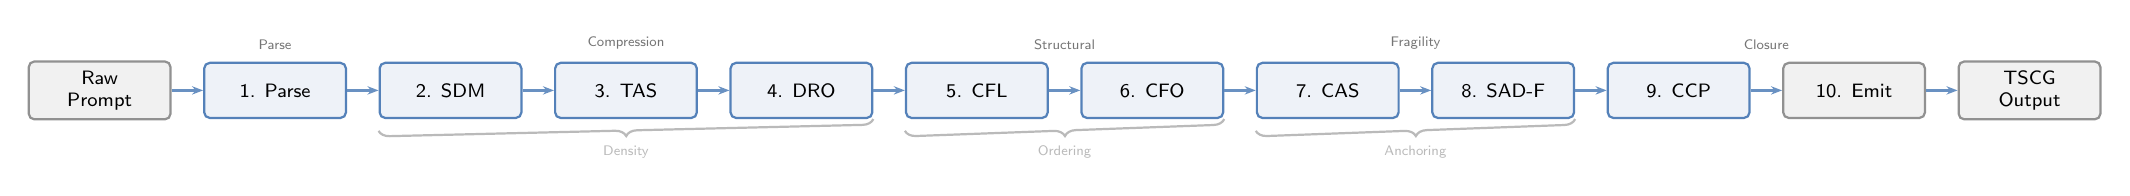
\begin{tikzpicture}[
    node distance=0.4cm,
    box/.style={
        rectangle,
        draw=tscgblue!80,
        fill=tscgblue!8,
        rounded corners=2pt,
        minimum height=0.7cm,
        minimum width=1.8cm,
        font=\scriptsize\sffamily,
        align=center,
        thick
    },
    iobox/.style={
        rectangle,
        draw=tscggray!80,
        fill=tscggray!10,
        rounded corners=2pt,
        minimum height=0.7cm,
        minimum width=1.8cm,
        font=\scriptsize\sffamily,
        align=center,
        thick
    },
    arr/.style={
        -{Stealth[length=4pt]},
        thick,
        tscgblue!70
    },
    phase/.style={
        font=\tiny\sffamily\color{tscggray},
        above=1pt
    }
]

% Input
\node[iobox] (input) {Raw\\Prompt};

% Phase 1: Parse
\node[box, right=of input] (parse) {1. Parse};

% Phase 2: Compression
\node[box, right=of parse] (sdm) {2. SDM};
\node[box, right=of sdm] (tas) {3. TAS};
\node[box, right=of tas] (dro) {4. DRO};

% Phase 3: Structural
\node[box, right=of dro] (cfl) {5. CFL};
\node[box, right=of cfl] (cfo) {6. CFO};

% Phase 4: Fragility
\node[box, right=of cfo] (cas) {7. CAS};
\node[box, right=of cas] (sadf) {8. SAD-F};

% Phase 5: Closure + Emit
\node[box, right=of sadf] (ccp) {9. CCP};
\node[iobox, right=of ccp] (emit) {10. Emit};

% Output
\node[iobox, right=of emit] (output) {TSCG\\Output};

% Arrows
\draw[arr] (input) -- (parse);
\draw[arr] (parse) -- (sdm);
\draw[arr] (sdm) -- (tas);
\draw[arr] (tas) -- (dro);
\draw[arr] (dro) -- (cfl);
\draw[arr] (cfl) -- (cfo);
\draw[arr] (cfo) -- (cas);
\draw[arr] (cas) -- (sadf);
\draw[arr] (sadf) -- (ccp);
\draw[arr] (ccp) -- (emit);
\draw[arr] (emit) -- (output);

% Phase labels
\node[phase] at (parse.north) {Parse};
\node[phase] at ($(sdm.north)!0.5!(dro.north)$) {Compression};
\node[phase] at ($(cfl.north)!0.5!(cfo.north)$) {Structural};
\node[phase] at ($(cas.north)!0.5!(sadf.north)$) {Fragility};
\node[phase] at ($(ccp.north)!0.5!(emit.north)$) {Closure};

% Phase grouping brackets
\draw[decorate, decoration={brace, amplitude=4pt, mirror}, tscggray!50, thick]
    (sdm.south west) ++(0,-0.15) -- (dro.south east |- sdm.south west) ++(0,-0.15)
    node[midway, below=4pt, font=\tiny\sffamily\color{tscggray}] {Density};

\draw[decorate, decoration={brace, amplitude=4pt, mirror}, tscggray!50, thick]
    (cfl.south west) ++(0,-0.15) -- (cfo.south east |- cfl.south west) ++(0,-0.15)
    node[midway, below=4pt, font=\tiny\sffamily\color{tscggray}] {Ordering};

\draw[decorate, decoration={brace, amplitude=4pt, mirror}, tscggray!50, thick]
    (cas.south west) ++(0,-0.15) -- (sadf.south east |- cas.south west) ++(0,-0.15)
    node[midway, below=4pt, font=\tiny\sffamily\color{tscggray}] {Anchoring};

\end{tikzpicture}
\caption{The TSCG 10-pass transform pipeline. Transforms execute in fixed order from left to right. The pipeline is organized into five phases: \emph{Parse} segments the input into semantic units; \emph{Compression} (SDM, TAS, DRO) removes filler and optimizes delimiters; \emph{Structural} (CFL, CFO) positions constraints and orders operations; \emph{Fragility} (CAS, SAD-F) scores and reinforces critical parameters; \emph{Closure} (CCP, Emit) appends the semantic closure block and generates the final output. Each transform is a pure function; the pipeline composition $\Pi = \tau_{10} \circ \cdots \circ \tau_1$ is deterministic.}
\label{fig:pipeline}
\end{figure*}


\subsection{Operator Taxonomy}

\begin{definition}[Token-Reducing Operators]
\label{def:token-reducing}
$\mathcal{T}_R = \{\text{SDM}, \text{DRO}, \text{TAS}, \text{CFL}\}$: each satisfies $|\tok(T_i(S))| \leq |\tok(S)|$.
\end{definition}

\begin{definition}[Structure-Reordering Operators]
\label{def:structure-reordering}
$\mathcal{T}_S = \{\text{CAS}, \text{CFO}\}$: preserve token count but change position order.
\end{definition}

\begin{definition}[Token-Expanding Operators]
\label{def:token-expanding}
$\mathcal{T}_E = \{\text{SAD}, \text{CCP}\}$: add tokens (anchor duplications, closure blocks) within budget.
\end{definition}

\begin{corollary}[Operator Interaction Effect]
\label{cor:interaction}
For models with ${<}$10B parameters, $\mathrm{Acc}(\mathcal{T}_R(S)) > \mathrm{Acc}((\mathcal{T}_R \cup \mathcal{T}_S)(S))$: adding structure-reordering operators to token-reducing operators \emph{degrades} accuracy.
Conservative profile ($\mathcal{T}_R$ only) is recommended below 10B.
\end{corollary}

\subsection{Compression Guarantee}

\begin{theorem}[Deterministic Compression Bound]
\label{thm:compression}
For a well-formed JSON-Schema tool collection $S$ with the TSCG pipeline $\Pi$:
\begin{equation}
  |\tok(\Pi(S))| \leq |\tok(S)| \cdot \Bigl(1 - \sum_{T_i \in \mathcal{T}_R} r_i \cdot f_i(S)\Bigr)
  \label{eq:compression-bound}
\end{equation}
where $r_i$ is the per-token reduction factor and $f_i(S)$ the fraction of tokens affected by operator $T_i$.
\end{theorem}

\begin{proof}[Proof sketch]
Each operator in $\mathcal{T}_R$ acts on disjoint token subsets (SDM: filler patterns; DRO: verbose delimiters; TAS: suboptimal tokenizer splits; CFL: positional overhead).
Structure-reordering operators preserve count; setting SAD-F budget $B{=}0$ excludes expansion.
Individual reductions compose additively.
Full proof in Appendix~E.
\end{proof}

\paragraph{Empirical validation.}
The bound predicts $\geq$51\% savings; empirically we observe 61\% (Scenario~A), 66\% (BFCL), and 75\% (tool descriptions)---conservative by 10--24\,pp due to the pessimistic disjoint-subset assumption.

\subsection{Scoring Metric}

All TAB results use a composite accuracy metric:
\begin{equation}
\text{Overall} = 0.6 \times \text{TSA} + 0.4 \times \text{Parameter\_F1}
\end{equation}
where TSA is tool selection accuracy and Parameter\_F1 measures parameter extraction quality.

\subsection{Compiler Characterization}

TSCG is a \emph{compiler}, not a search-based optimizer.
The pipeline $\Pi = \tau_{10} \circ \cdots \circ \tau_1$ applies 10 deterministic transforms in fixed order: same input always produces the same output.
No model access is required.
This distinguishes TSCG from DSPy~\cite{khattab2023dspy} (search-based, non-deterministic), TextGrad~\cite{yuksekgonul2024textgrad} (gradient-based, requires model access), and LLMLingua~\cite{pan2024llmlingua2} (requires GPU model inference, non-deterministic).
TSCG executes in ${<}$1\,ms on commodity hardware; LLMLingua-2 requires 42.5\,s on the same prompts (${\sim}$40{,}000$\times$ slower).

\section{Theoretical Foundations}
\label{sec:theoretical}

% Full proofs and extended formal analysis relocated to Appendix~E.

We connect TSCG's operators to three foundational properties of causal autoregressive transformers.

\subsection{Causal Attention and Information Flow}

In a standard autoregressive transformer~\cite{vaswani2017attention}, attention at layer $\ell$ satisfies $\attn^{(\ell)}(i, j) = 0$ for $j > i$ (causal mask), creating asymmetric information flow: early tokens cannot access later ones.

\textbf{Implication for CFO.} If step $o_2$ depends on $o_1$ but $o_1$ appears \emph{after} $o_2$, the model must rely on parametric knowledge rather than direct attention.
CFO ensures $\pos(o_1) < \pos(o_2)$, guaranteeing prerequisites are causally accessible.

\textbf{Implication for CAS.} Total attention to position $i$ follows a U-shaped distribution~\cite{xiao2023efficient}: positions near 0 and $n$ receive disproportionate attention, while middle positions form an ``attention valley.''
CAS places high-fragility tools at positions~0 and~$n$.

\subsection{Attention Sink Exploitation}

The attention sink phenomenon~\cite{xiao2023efficient}---position~0 receives $\attn(i, 0) > 1/i$ for most $i$ and layers---provides a natural amplification mechanism.

\textbf{Implication for CFL.} Placing the output constraint at position~0 ensures it receives elevated attention from every subsequent token.
Combined with CCP/SAD-F at position~$n$ (recency bias), this creates a ``bookend'' strategy: critical information occupies both extremes of the attention distribution.

\subsection{BPE Non-Monotonicity}

\begin{theorem}[Tokenization Non-Monotonicity]
\label{thm:non-monotonicity}
For BPE tokenizer $\mathcal{T}$ and strings $s_1, s_2$ with $|s_1|_\text{chars} < |s_2|_\text{chars}$, it is not necessarily the case that $|\tok(s_1)| < |\tok(s_2)|$.
\end{theorem}

TAS exploits this by selecting surface forms aligned with learned BPE merges, achieving token reduction without semantic change.
Proof in Appendix~E.

\subsection{Attention Dilution and SDM}

\begin{proposition}[SDM Improves Effective Attention]
\label{prop:sdm-attention}
Removing $k$ filler tokens from a prompt of length $n$ increases average effective attention per semantic atom by at least $n/(n-k)$.
\end{proposition}

This follows from softmax normalization: filler tokens compete for attention weight with semantic tokens.
SDM removes this competition, providing formal justification beyond token cost savings.

\subsection{Fragility and Causal Accessibility}

\begin{definition}[Causal Accessibility]
\label{def:causal-accessibility}
$\mathcal{A}(a) = \frac{1}{L} \sum_{\ell=1}^{L} \attn^{(\ell)}(n, i)$: average attention from the generation position to atom $a$ at position $i$.
\end{definition}

\begin{definition}[Fragility]
\label{def:fragility-gap}
An atom $a$ is fragile when importance exceeds accessibility: $\fragility(a) \propto \text{importance}(a) - \mathcal{A}(a)$.
\end{definition}

High-importance, low-accessibility atoms are the targets for CAS reordering and SAD-F duplication.
Budget-constrained duplication is preferable to naive repetition because duplicating all atoms would increase length and dilute attention (Proposition~\ref{prop:sdm-attention}).

\section{Experiments}
\label{sec:experiments}

% Pre-TAB evaluation (19 core tasks, 6 strategies, 11 runs, domain benchmarks,
% multi-model protocol, LLMLingua comparison) relocated to Appendix~\ref{app:pre-tab}.

\subsection{TAB: TSCG-Agentic-Bench}
\label{sec:tab-benchmark}

TAB is the first benchmark measuring tool-schema compression effects on LLM tool-use, comprising five scenarios across ${\sim}$13{,}000 API calls and 12~models (4B--32B local + 3~frontier; Table~\ref{tab:tab-overview}).
Each scenario compares Natural (uncompressed JSON), TSCG, and TSCG+SAD across four task categories (single\_tool, multi\_tool, parameter\_extraction, no\_tool).
Overall accuracy = $0.6 \times \text{TSA} + 0.4 \times \text{PF1}$.

\begin{table}[h]
\centering
\small
\caption{TAB: five scenarios, ${\sim}$13{,}000 calls.}
\label{tab:tab-overview}
\begin{tabular}{llrr}
\toprule
\textbf{Sc.} & \textbf{Focus} & \textbf{Tools} & \textbf{Calls} \\
\midrule
A & Claude Code (16 real tools) & 16 & ${\sim}$540 \\
B & MCP Servers & 43 & ${\sim}$2{,}700 \\
C & Scaling (25--100 tools) & var. & ${\sim}$1{,}080 \\
D & Small models $\times$ 7 configs & var. & ${\sim}$5{,}000 \\
E & Multi-collection & 57 & ${\sim}$540 \\
\bottomrule
\end{tabular}
\end{table}

\paragraph{Scenario A (Claude Code).}
Claude Sonnet~4 achieves 68.9\% natural (JSON), 78.9\% TSCG (50.1\% savings, ARR~115\%).
Text-mode: TSCG 87.8\% vs.\ 76.9\% natural---$+$10.9\,pp genuine compression.
GPT-5.2 shows the largest frontier effect: $+$24.4\,pp (CI~[$+$15.0, $+$33.9], $d{=}0.54$).

\paragraph{Scenario D (Small-Model Unlock).}
Seven models (4B--14B) at 3--50 tools: JSON-baseline accuracy 0--49\% at $>$15 tools; TSCG recovers to 65--90\% (Table~\ref{tab:small-model}).
Models exceeding the 65\% threshold at 50~tools rise from 4/7 to 7/7 (Figure~\ref{fig:capability-heatmap}).

\begin{table}[h]
\centering
\small
\caption{Scenario D: accuracy at 20 and 50 tools.}
\label{tab:small-model}
\begin{tabular}{lccccc}
\toprule
\textbf{Model} & \multicolumn{2}{c}{\textbf{20 Tools}} & \multicolumn{2}{c}{\textbf{50 Tools}} & \textbf{Shift} \\
\cmidrule(lr){2-3} \cmidrule(lr){4-5}
& Nat. & TSCG & Nat. & TSCG & \\
\midrule
Phi-4 14B    & 0.0  & 84.4 & 0.0  & 90.3 & 3$\to$50  \\
Mistral 7B   & 35.0 & 80.1 & 30.0 & 65.0 & 20$\to$50 \\
Gemma 3 4B   & 49.9 & 67.0 & 24.3 & 87.4 & 15$\to$50 \\
Gemma 3 12B  & 85.0 & 95.0 & 85.0 & 98.0 & ---  \\
Llama 3.1 8B & 78.4 & 81.0 & 75.1 & 86.3 & ---  \\
Qwen3 4B     & 44.3 & 69.3 & 90.0 & 75.0 & volatile  \\
Qwen3 14B    & 90.2 & 84.1 & 94.6 & 89.6 & --- \\
\bottomrule
\end{tabular}
\end{table}

% fig2-capability-heatmap.tex -- TSCG Delta heatmap: Model x Tool Count
% Included via % fig2-capability-heatmap.tex -- TSCG Delta heatmap: Model x Tool Count
% Included via \input{figures/fig2-capability-heatmap} from main.tex
% Requires: tikz, pgfplots (compat=1.18), xcolor, custom tscg* colors from main.tex
\begin{figure*}[t]
\centering
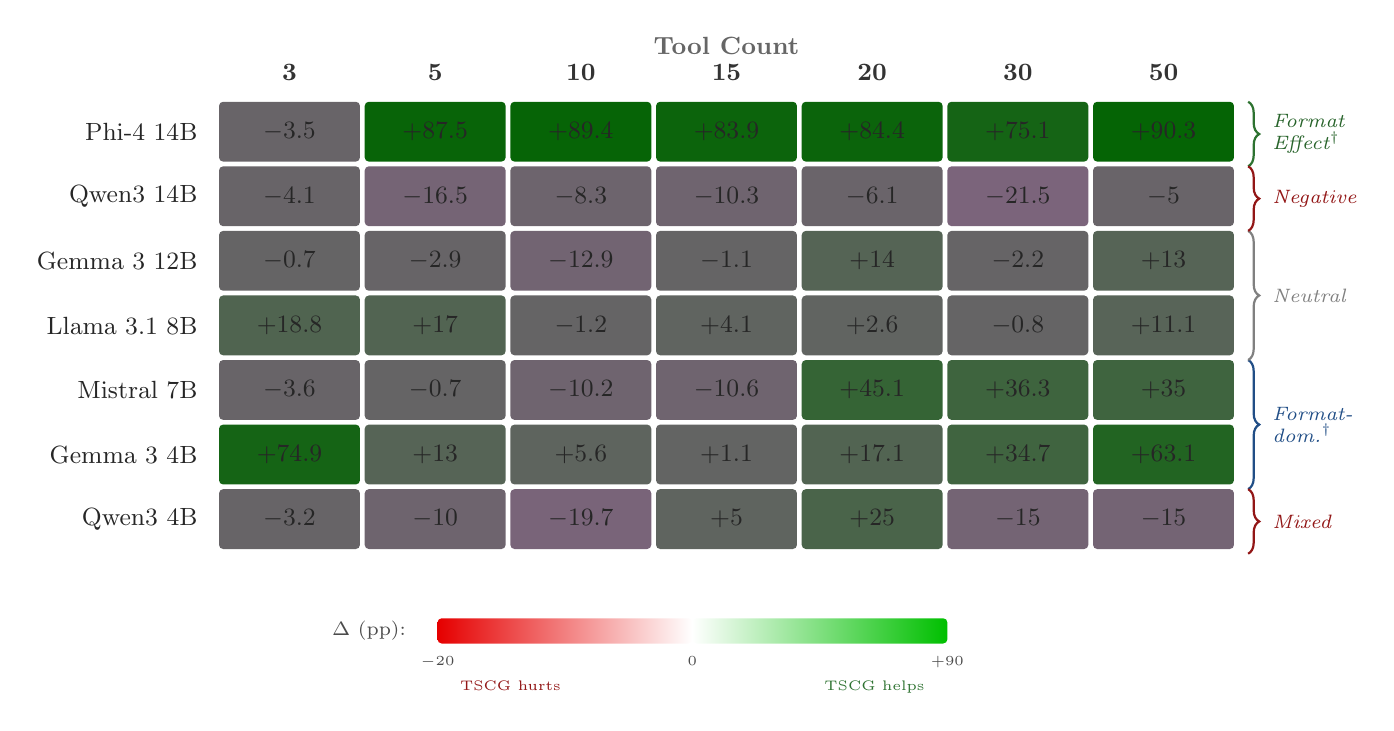
\begin{tikzpicture}[
    % --- cell dimensions ---
    cell width/.store in=\cellw, cell width=1.85cm,
    cell height/.store in=\cellh, cell height=0.82cm,
]

% =========================================================================
%  Color mapping: red (negative) -> white (0) -> green (positive)
%  Clamp range to [-25, +95] for visual balance
% =========================================================================
\pgfmathdeclarefunction{heatR}{1}{%
    \pgfmathparse{%
        (#1 < 0) ? (100) :                              % negative -> red channel high
        (#1 >= 0 && #1 <= 95) ? (100 - #1*1.05) :       % positive -> fade red out
        (0)                                              % saturated green
    }%
}
\pgfmathdeclarefunction{heatG}{1}{%
    \pgfmathparse{%
        (#1 < -25) ? (0) :                              % deep negative -> no green
        (#1 >= -25 && #1 < 0) ? (100 + #1*4) :          % negative -> dim green
        (#1 >= 0) ? (100) :                              % positive -> green channel high
        (0)
    }%
}
\pgfmathdeclarefunction{heatB}{1}{%
    \pgfmathparse{%
        (#1 < 0) ? (100 + #1*4) :                       % negative -> dim blue
        (#1 >= 0 && #1 <= 95) ? (100 - #1*1.05) :       % positive -> fade blue out
        (0)
    }%
}

% =========================================================================
%  Helper: draw one heatmap cell
%    #1 = column index (0-based), #2 = row index (0-based), #3 = delta value
% =========================================================================
\newcommand{\hcell}[3]{%
    \pgfmathsetmacro{\cR}{heatR(#3)}%
    \pgfmathsetmacro{\cG}{heatG(#3)}%
    \pgfmathsetmacro{\cB}{heatB(#3)}%
    \definecolor{cellcol}{RGB}{\cR,\cG,\cB}%
    % choose black text on light cells, white on dark cells
    \pgfmathsetmacro{\lum}{0.299*\cR + 0.587*\cG + 0.114*\cB}%
    \pgfmathparse{\lum > 55 ? 1 : 0}%
    \ifnum\pgfmathresult=1
        \colorlet{txtcol}{black!85}%
    \else
        \colorlet{txtcol}{white}%
    \fi
    % draw filled rectangle
    \fill[cellcol, rounded corners=1.5pt]
        ({#1*\cellw}, {#2*\cellh})
        rectangle
        ({#1*\cellw + \cellw - 0.06cm}, {#2*\cellh + \cellh - 0.06cm});
    % print value
    \node[font=\small\bfseries, text=txtcol]
        at ({#1*\cellw + \cellw/2 - 0.03cm}, {#2*\cellh + \cellh/2 - 0.03cm})
        {\pgfmathprintnumber[fixed, precision=1, showpos]{#3}};
}

% =========================================================================
%  Data matrix  (row 0 = bottom = Qwen3 4B, row 6 = top = Phi-4 14B)
%  Sorted by parameter size ascending (bottom to top)
%  Columns: 3, 5, 10, 15, 20, 30, 50
% =========================================================================

% Row 0: Qwen3 4B
\hcell{0}{0}{-3.2}   \hcell{1}{0}{-10.0}  \hcell{2}{0}{-19.7}
\hcell{3}{0}{5.0}    \hcell{4}{0}{25.0}   \hcell{5}{0}{-15.0}  \hcell{6}{0}{-15.0}

% Row 1: Gemma 3 4B
\hcell{0}{1}{74.9}   \hcell{1}{1}{13.0}   \hcell{2}{1}{5.6}
\hcell{3}{1}{1.1}    \hcell{4}{1}{17.1}   \hcell{5}{1}{34.7}   \hcell{6}{1}{63.1}

% Row 2: Mistral 7B
\hcell{0}{2}{-3.6}   \hcell{1}{2}{-0.7}   \hcell{2}{2}{-10.2}
\hcell{3}{2}{-10.6}  \hcell{4}{2}{45.1}   \hcell{5}{2}{36.3}   \hcell{6}{2}{35.0}

% Row 3: Llama 3.1 8B
\hcell{0}{3}{18.8}   \hcell{1}{3}{17.0}   \hcell{2}{3}{-1.2}
\hcell{3}{3}{4.1}    \hcell{4}{3}{2.6}    \hcell{5}{3}{-0.8}   \hcell{6}{3}{11.1}

% Row 4: Gemma 3 12B
\hcell{0}{4}{-0.7}   \hcell{1}{4}{-2.9}   \hcell{2}{4}{-12.9}
\hcell{3}{4}{-1.1}   \hcell{4}{4}{14.0}   \hcell{5}{4}{-2.2}   \hcell{6}{4}{13.0}

% Row 5: Qwen3 14B
\hcell{0}{5}{-4.1}   \hcell{1}{5}{-16.5}  \hcell{2}{5}{-8.3}
\hcell{3}{5}{-10.3}  \hcell{4}{5}{-6.1}   \hcell{5}{5}{-21.5}  \hcell{6}{5}{-5.0}

% Row 6: Phi-4 14B
\hcell{0}{6}{-3.5}   \hcell{1}{6}{87.5}   \hcell{2}{6}{89.4}
\hcell{3}{6}{83.9}   \hcell{4}{6}{84.4}   \hcell{5}{6}{75.1}   \hcell{6}{6}{90.3}

% =========================================================================
%  Column headers (tool counts)
% =========================================================================
\foreach \col/\lab in {0/3, 1/5, 2/10, 3/15, 4/20, 5/30, 6/50} {
    \node[font=\small\bfseries, text=black!80, anchor=south]
        at ({\col*\cellw + \cellw/2 - 0.03cm}, {7*\cellh + 0.08cm}) {\lab};
}
% axis label
\node[font=\small\bfseries, text=black!60, anchor=south]
    at ({3*\cellw + \cellw/2 - 0.03cm}, {7*\cellh + 0.42cm}) {Tool Count};

% =========================================================================
%  Row labels (model names, left side)
% =========================================================================
\foreach \row/\lab in {
    0/{Qwen3 4B},
    1/{Gemma 3 4B},
    2/{Mistral 7B},
    3/{Llama 3.1 8B},
    4/{Gemma 3 12B},
    5/{Qwen3 14B},
    6/{Phi-4 14B}%
} {
    \node[font=\small, anchor=east, text=black!85]
        at ({-0.15cm}, {\row*\cellh + \cellh/2 - 0.03cm}) {\lab};
}

% =========================================================================
%  Cluster annotations (right side, with decorations.pathreplacing braces)
% =========================================================================

% Cluster 1: "Format Effect" -- Phi-4 (row 6) -- E1 confirmed: JSON->text translation
\draw[decorate, decoration={brace, amplitude=4pt, mirror},
      tscggreen!80!black, line width=0.8pt]
    ({6*\cellw + \cellw + 0.12cm}, {6*\cellh - 0.06cm})
    -- ({6*\cellw + \cellw + 0.12cm}, {6*\cellh + \cellh - 0.06cm})
    node[midway, right=5pt, font=\scriptsize\itshape, text=tscggreen!70!black,
         align=left] {Format\\Effect$^\dagger$};

% Cluster 2: "Format-dominated" -- Mistral + Gemma 4B (rows 1-2) -- E4 confirmed
\draw[decorate, decoration={brace, amplitude=4pt, mirror},
      tscgblue!80!black, line width=0.8pt]
    ({6*\cellw + \cellw + 0.12cm}, {1*\cellh - 0.06cm})
    -- ({6*\cellw + \cellw + 0.12cm}, {2*\cellh + \cellh - 0.06cm})
    node[midway, right=5pt, font=\scriptsize\itshape, text=tscgblue!80!black,
         align=left] {Format-\\dom.$^\dagger$};

% Cluster 3: "Neutral" -- Llama + Gemma 12B (rows 3-4)
\draw[decorate, decoration={brace, amplitude=4pt, mirror},
      black!50, line width=0.8pt]
    ({6*\cellw + \cellw + 0.12cm}, {3*\cellh - 0.06cm})
    -- ({6*\cellw + \cellw + 0.12cm}, {4*\cellh + \cellh - 0.06cm})
    node[midway, right=5pt, font=\scriptsize\itshape, text=black!50,
         align=left] {Neutral};

% Cluster 4: "Negative" -- Qwen3 14B + Qwen3 4B (rows 0, 5)
\draw[decorate, decoration={brace, amplitude=4pt, mirror},
      tscgred!80!black, line width=0.8pt]
    ({6*\cellw + \cellw + 0.12cm}, {5*\cellh - 0.06cm})
    -- ({6*\cellw + \cellw + 0.12cm}, {5*\cellh + \cellh - 0.06cm})
    node[midway, right=5pt, font=\scriptsize\itshape, text=tscgred!80!black,
         align=left] {Negative};

\draw[decorate, decoration={brace, amplitude=4pt, mirror},
      tscgred!80!black, line width=0.8pt]
    ({6*\cellw + \cellw + 0.12cm}, {0*\cellh - 0.06cm})
    -- ({6*\cellw + \cellw + 0.12cm}, {0*\cellh + \cellh - 0.06cm})
    node[midway, right=5pt, font=\scriptsize\itshape, text=tscgred!80!black,
         align=left] {Mixed};

% =========================================================================
%  Color legend (horizontal bar below the matrix)
% =========================================================================
\begin{scope}[yshift=-1.2cm]
    % gradient bar
    \shade[left color=red!90!black, right color=white, rounded corners=1.5pt]
        ({1.5*\cellw}, 0) rectangle ({3.25*\cellw}, 0.32cm);
    \shade[left color=white, right color=green!75!black, rounded corners=1.5pt]
        ({3.25*\cellw}, 0) rectangle ({5.0*\cellw}, 0.32cm);
    % ticks
    \node[font=\tiny, anchor=north, text=black!70] at ({1.5*\cellw}, -0.04cm) {$-20$};
    \node[font=\tiny, anchor=north, text=black!70] at ({3.25*\cellw}, -0.04cm) {$0$};
    \node[font=\tiny, anchor=north, text=black!70] at ({5.0*\cellw}, -0.04cm) {$+90$};
    % label
    \node[font=\scriptsize, anchor=east, text=black!70] at ({1.35*\cellw}, 0.16cm)
        {$\Delta$ (pp):};
    % semantic labels
    \node[font=\tiny, text=tscgred!80!black, anchor=north] at ({2.0*\cellw}, -0.35cm)
        {TSCG hurts};
    \node[font=\tiny, text=tscggreen!80!black, anchor=north] at ({4.5*\cellw}, -0.35cm)
        {TSCG helps};
\end{scope}

\end{tikzpicture}
\caption{TSCG delta heatmap ($\Delta = \text{TSCG accuracy} - \text{JSON-baseline accuracy}$, in percentage points) across seven models and seven tool-count conditions. Green cells indicate conditions where TSCG improves over JSON schemas; red cells indicate degradation. Five behavioral clusters emerge: \emph{Format Effect}$^\dagger$---Phi-4's +75--90\,pp gains are JSON$\to$text translation, not compression benefit (\S\ref{sec:format-effect}); \emph{Format-dominated}$^\dagger$---Mistral and Gemma~4B show large deltas driven primarily by format translation; \emph{Neutral}---Llama~3.1~8B and Gemma~3~12B show modest mixed effects; \emph{Negative}---Qwen3~14B shows uniform degradation ($-$4 to $-$22\,pp); \emph{Mixed}---Qwen3~4B exhibits chaotic response. $^\dagger$E1/E4 text-baseline experiments confirm format contribution (\S\ref{sec:experiments}).}
\label{fig:capability-heatmap}
\end{figure*}
 from main.tex
% Requires: tikz, pgfplots (compat=1.18), xcolor, custom tscg* colors from main.tex
\begin{figure*}[t]
\centering
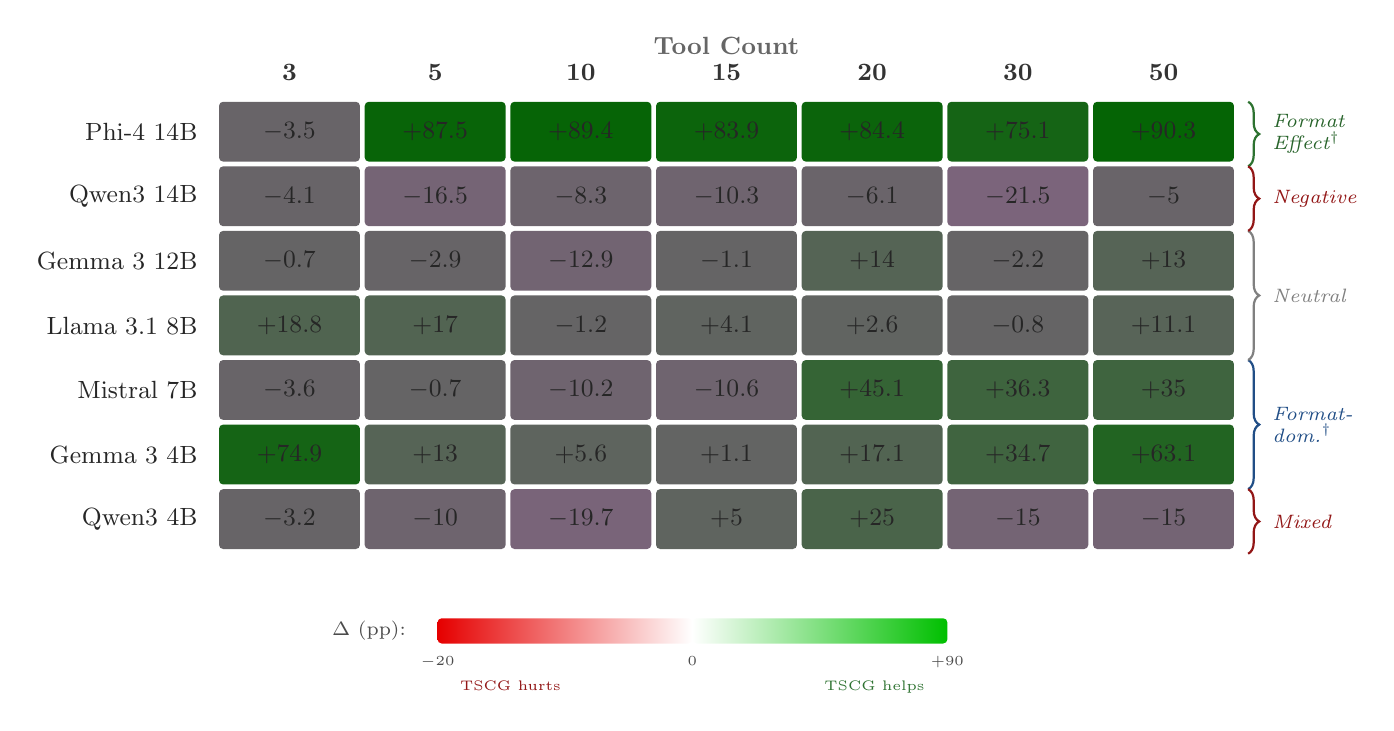
\begin{tikzpicture}[
    % --- cell dimensions ---
    cell width/.store in=\cellw, cell width=1.85cm,
    cell height/.store in=\cellh, cell height=0.82cm,
]

% =========================================================================
%  Color mapping: red (negative) -> white (0) -> green (positive)
%  Clamp range to [-25, +95] for visual balance
% =========================================================================
\pgfmathdeclarefunction{heatR}{1}{%
    \pgfmathparse{%
        (#1 < 0) ? (100) :                              % negative -> red channel high
        (#1 >= 0 && #1 <= 95) ? (100 - #1*1.05) :       % positive -> fade red out
        (0)                                              % saturated green
    }%
}
\pgfmathdeclarefunction{heatG}{1}{%
    \pgfmathparse{%
        (#1 < -25) ? (0) :                              % deep negative -> no green
        (#1 >= -25 && #1 < 0) ? (100 + #1*4) :          % negative -> dim green
        (#1 >= 0) ? (100) :                              % positive -> green channel high
        (0)
    }%
}
\pgfmathdeclarefunction{heatB}{1}{%
    \pgfmathparse{%
        (#1 < 0) ? (100 + #1*4) :                       % negative -> dim blue
        (#1 >= 0 && #1 <= 95) ? (100 - #1*1.05) :       % positive -> fade blue out
        (0)
    }%
}

% =========================================================================
%  Helper: draw one heatmap cell
%    #1 = column index (0-based), #2 = row index (0-based), #3 = delta value
% =========================================================================
\newcommand{\hcell}[3]{%
    \pgfmathsetmacro{\cR}{heatR(#3)}%
    \pgfmathsetmacro{\cG}{heatG(#3)}%
    \pgfmathsetmacro{\cB}{heatB(#3)}%
    \definecolor{cellcol}{RGB}{\cR,\cG,\cB}%
    % choose black text on light cells, white on dark cells
    \pgfmathsetmacro{\lum}{0.299*\cR + 0.587*\cG + 0.114*\cB}%
    \pgfmathparse{\lum > 55 ? 1 : 0}%
    \ifnum\pgfmathresult=1
        \colorlet{txtcol}{black!85}%
    \else
        \colorlet{txtcol}{white}%
    \fi
    % draw filled rectangle
    \fill[cellcol, rounded corners=1.5pt]
        ({#1*\cellw}, {#2*\cellh})
        rectangle
        ({#1*\cellw + \cellw - 0.06cm}, {#2*\cellh + \cellh - 0.06cm});
    % print value
    \node[font=\small\bfseries, text=txtcol]
        at ({#1*\cellw + \cellw/2 - 0.03cm}, {#2*\cellh + \cellh/2 - 0.03cm})
        {\pgfmathprintnumber[fixed, precision=1, showpos]{#3}};
}

% =========================================================================
%  Data matrix  (row 0 = bottom = Qwen3 4B, row 6 = top = Phi-4 14B)
%  Sorted by parameter size ascending (bottom to top)
%  Columns: 3, 5, 10, 15, 20, 30, 50
% =========================================================================

% Row 0: Qwen3 4B
\hcell{0}{0}{-3.2}   \hcell{1}{0}{-10.0}  \hcell{2}{0}{-19.7}
\hcell{3}{0}{5.0}    \hcell{4}{0}{25.0}   \hcell{5}{0}{-15.0}  \hcell{6}{0}{-15.0}

% Row 1: Gemma 3 4B
\hcell{0}{1}{74.9}   \hcell{1}{1}{13.0}   \hcell{2}{1}{5.6}
\hcell{3}{1}{1.1}    \hcell{4}{1}{17.1}   \hcell{5}{1}{34.7}   \hcell{6}{1}{63.1}

% Row 2: Mistral 7B
\hcell{0}{2}{-3.6}   \hcell{1}{2}{-0.7}   \hcell{2}{2}{-10.2}
\hcell{3}{2}{-10.6}  \hcell{4}{2}{45.1}   \hcell{5}{2}{36.3}   \hcell{6}{2}{35.0}

% Row 3: Llama 3.1 8B
\hcell{0}{3}{18.8}   \hcell{1}{3}{17.0}   \hcell{2}{3}{-1.2}
\hcell{3}{3}{4.1}    \hcell{4}{3}{2.6}    \hcell{5}{3}{-0.8}   \hcell{6}{3}{11.1}

% Row 4: Gemma 3 12B
\hcell{0}{4}{-0.7}   \hcell{1}{4}{-2.9}   \hcell{2}{4}{-12.9}
\hcell{3}{4}{-1.1}   \hcell{4}{4}{14.0}   \hcell{5}{4}{-2.2}   \hcell{6}{4}{13.0}

% Row 5: Qwen3 14B
\hcell{0}{5}{-4.1}   \hcell{1}{5}{-16.5}  \hcell{2}{5}{-8.3}
\hcell{3}{5}{-10.3}  \hcell{4}{5}{-6.1}   \hcell{5}{5}{-21.5}  \hcell{6}{5}{-5.0}

% Row 6: Phi-4 14B
\hcell{0}{6}{-3.5}   \hcell{1}{6}{87.5}   \hcell{2}{6}{89.4}
\hcell{3}{6}{83.9}   \hcell{4}{6}{84.4}   \hcell{5}{6}{75.1}   \hcell{6}{6}{90.3}

% =========================================================================
%  Column headers (tool counts)
% =========================================================================
\foreach \col/\lab in {0/3, 1/5, 2/10, 3/15, 4/20, 5/30, 6/50} {
    \node[font=\small\bfseries, text=black!80, anchor=south]
        at ({\col*\cellw + \cellw/2 - 0.03cm}, {7*\cellh + 0.08cm}) {\lab};
}
% axis label
\node[font=\small\bfseries, text=black!60, anchor=south]
    at ({3*\cellw + \cellw/2 - 0.03cm}, {7*\cellh + 0.42cm}) {Tool Count};

% =========================================================================
%  Row labels (model names, left side)
% =========================================================================
\foreach \row/\lab in {
    0/{Qwen3 4B},
    1/{Gemma 3 4B},
    2/{Mistral 7B},
    3/{Llama 3.1 8B},
    4/{Gemma 3 12B},
    5/{Qwen3 14B},
    6/{Phi-4 14B}%
} {
    \node[font=\small, anchor=east, text=black!85]
        at ({-0.15cm}, {\row*\cellh + \cellh/2 - 0.03cm}) {\lab};
}

% =========================================================================
%  Cluster annotations (right side, with decorations.pathreplacing braces)
% =========================================================================

% Cluster 1: "Format Effect" -- Phi-4 (row 6) -- E1 confirmed: JSON->text translation
\draw[decorate, decoration={brace, amplitude=4pt, mirror},
      tscggreen!80!black, line width=0.8pt]
    ({6*\cellw + \cellw + 0.12cm}, {6*\cellh - 0.06cm})
    -- ({6*\cellw + \cellw + 0.12cm}, {6*\cellh + \cellh - 0.06cm})
    node[midway, right=5pt, font=\scriptsize\itshape, text=tscggreen!70!black,
         align=left] {Format\\Effect$^\dagger$};

% Cluster 2: "Format-dominated" -- Mistral + Gemma 4B (rows 1-2) -- E4 confirmed
\draw[decorate, decoration={brace, amplitude=4pt, mirror},
      tscgblue!80!black, line width=0.8pt]
    ({6*\cellw + \cellw + 0.12cm}, {1*\cellh - 0.06cm})
    -- ({6*\cellw + \cellw + 0.12cm}, {2*\cellh + \cellh - 0.06cm})
    node[midway, right=5pt, font=\scriptsize\itshape, text=tscgblue!80!black,
         align=left] {Format-\\dom.$^\dagger$};

% Cluster 3: "Neutral" -- Llama + Gemma 12B (rows 3-4)
\draw[decorate, decoration={brace, amplitude=4pt, mirror},
      black!50, line width=0.8pt]
    ({6*\cellw + \cellw + 0.12cm}, {3*\cellh - 0.06cm})
    -- ({6*\cellw + \cellw + 0.12cm}, {4*\cellh + \cellh - 0.06cm})
    node[midway, right=5pt, font=\scriptsize\itshape, text=black!50,
         align=left] {Neutral};

% Cluster 4: "Negative" -- Qwen3 14B + Qwen3 4B (rows 0, 5)
\draw[decorate, decoration={brace, amplitude=4pt, mirror},
      tscgred!80!black, line width=0.8pt]
    ({6*\cellw + \cellw + 0.12cm}, {5*\cellh - 0.06cm})
    -- ({6*\cellw + \cellw + 0.12cm}, {5*\cellh + \cellh - 0.06cm})
    node[midway, right=5pt, font=\scriptsize\itshape, text=tscgred!80!black,
         align=left] {Negative};

\draw[decorate, decoration={brace, amplitude=4pt, mirror},
      tscgred!80!black, line width=0.8pt]
    ({6*\cellw + \cellw + 0.12cm}, {0*\cellh - 0.06cm})
    -- ({6*\cellw + \cellw + 0.12cm}, {0*\cellh + \cellh - 0.06cm})
    node[midway, right=5pt, font=\scriptsize\itshape, text=tscgred!80!black,
         align=left] {Mixed};

% =========================================================================
%  Color legend (horizontal bar below the matrix)
% =========================================================================
\begin{scope}[yshift=-1.2cm]
    % gradient bar
    \shade[left color=red!90!black, right color=white, rounded corners=1.5pt]
        ({1.5*\cellw}, 0) rectangle ({3.25*\cellw}, 0.32cm);
    \shade[left color=white, right color=green!75!black, rounded corners=1.5pt]
        ({3.25*\cellw}, 0) rectangle ({5.0*\cellw}, 0.32cm);
    % ticks
    \node[font=\tiny, anchor=north, text=black!70] at ({1.5*\cellw}, -0.04cm) {$-20$};
    \node[font=\tiny, anchor=north, text=black!70] at ({3.25*\cellw}, -0.04cm) {$0$};
    \node[font=\tiny, anchor=north, text=black!70] at ({5.0*\cellw}, -0.04cm) {$+90$};
    % label
    \node[font=\scriptsize, anchor=east, text=black!70] at ({1.35*\cellw}, 0.16cm)
        {$\Delta$ (pp):};
    % semantic labels
    \node[font=\tiny, text=tscgred!80!black, anchor=north] at ({2.0*\cellw}, -0.35cm)
        {TSCG hurts};
    \node[font=\tiny, text=tscggreen!80!black, anchor=north] at ({4.5*\cellw}, -0.35cm)
        {TSCG helps};
\end{scope}

\end{tikzpicture}
\caption{TSCG delta heatmap ($\Delta = \text{TSCG accuracy} - \text{JSON-baseline accuracy}$, in percentage points) across seven models and seven tool-count conditions. Green cells indicate conditions where TSCG improves over JSON schemas; red cells indicate degradation. Five behavioral clusters emerge: \emph{Format Effect}$^\dagger$---Phi-4's +75--90\,pp gains are JSON$\to$text translation, not compression benefit (\S\ref{sec:format-effect}); \emph{Format-dominated}$^\dagger$---Mistral and Gemma~4B show large deltas driven primarily by format translation; \emph{Neutral}---Llama~3.1~8B and Gemma~3~12B show modest mixed effects; \emph{Negative}---Qwen3~14B shows uniform degradation ($-$4 to $-$22\,pp); \emph{Mixed}---Qwen3~4B exhibits chaotic response. $^\dagger$E1/E4 text-baseline experiments confirm format contribution (\S\ref{sec:experiments}).}
\label{fig:capability-heatmap}
\end{figure*}


N1 extends to 30B: Mistral-Small~24B ($-$1.1\,pp, Class~3); Qwen2.5-Coder~32B ($-$4.7\,pp, Class~4)---Qwen sensitivity persists across sizes.

\subsection{Format Translation vs.\ Compression (E4)}
\label{sec:format-effect}

E4 decomposes TSCG's JSON-baseline gains into format gain (text$-$JSON) and compression gain (TSCG$-$text) across six small models (2{,}520 Ollama calls; Table~\ref{tab:e4-decomposition}).

\begin{table}[h]
\centering
\small
\caption{E4: format vs.\ compression decomposition. No small model shows genuine compression.}
\label{tab:e4-decomposition}
\begin{tabular}{lrrr}
\toprule
\textbf{Model} & \textbf{Format $\Delta$} & \textbf{Compr.\ $\Delta$} & \textbf{Class} \\
\midrule
Phi-4 14B    & $+$92.0 & $-$7.0  & 1: Format \\
Mistral 7B   & $+$44.6 & $-$7.4  & 1: Format \\
Gemma 3 4B   & $+$47.3 & $-$8.9  & 1: Format \\
Qwen3 4B     & $+$16.7 & $-$23.4 & 1: Format \\
Llama 3.1 8B & $+$5.6  & $+$0.3  & 3: Neutral \\
Gemma 3 12B  & $+$9.2  & $-$0.9  & 3: Neutral \\
\bottomrule
\end{tabular}
\end{table}

TSCG's gains on small models arise from format translation (JSON$\to$text), not structural compression.
Since every production API transmits JSON, this translation \emph{is} the needed intervention.
Naive truncation outperforms TSCG in hypothetical text-mode (mean $+$10.6\,pp), but no production framework offers text-mode tools.

\subsection{R\textsuperscript{2} Decomposition and Naive Truncation}
\label{sec:correlation-thesis}

The predictive regression ($n{=}49$, 7~models $\times$ 7~sizes) yields:
\begin{equation}
\Delta_\text{TSCG} \approx -0.93 \times \text{Acc}_\text{JSON} + 0.76, \quad R^2 = 0.88
\label{eq:correlation}
\end{equation}
Against text baselines (E4): $R^2$ collapses to 0.03 ($p{=}0.24$)---a 97\% drop confirming format sensitivity, not compression (Figure~\ref{fig:natural-vs-delta}).
LOO RMSE = 12.8\,pp (detail in Appendix~\ref{app:loo-details}).

% fig8-natural-vs-delta.tex -- Dual-panel scatter: R² decomposition
% Panel A: JSON baseline (R²=0.88), Panel B: Text baseline (R²=0.03)
% KEY FINDING: 97% of R² vanishes when format confound is removed.
% n=49 per panel (7 models × 7 catalog sizes: 3,5,10,15,20,30,50)
% Included via % fig8-natural-vs-delta.tex -- Dual-panel scatter: R² decomposition
% Panel A: JSON baseline (R²=0.88), Panel B: Text baseline (R²=0.03)
% KEY FINDING: 97% of R² vanishes when format confound is removed.
% n=49 per panel (7 models × 7 catalog sizes: 3,5,10,15,20,30,50)
% Included via \input{figures/fig8-natural-vs-delta} from main.tex
\begin{figure*}[t]
\centering
\begin{subfigure}[t]{0.48\textwidth}
\centering
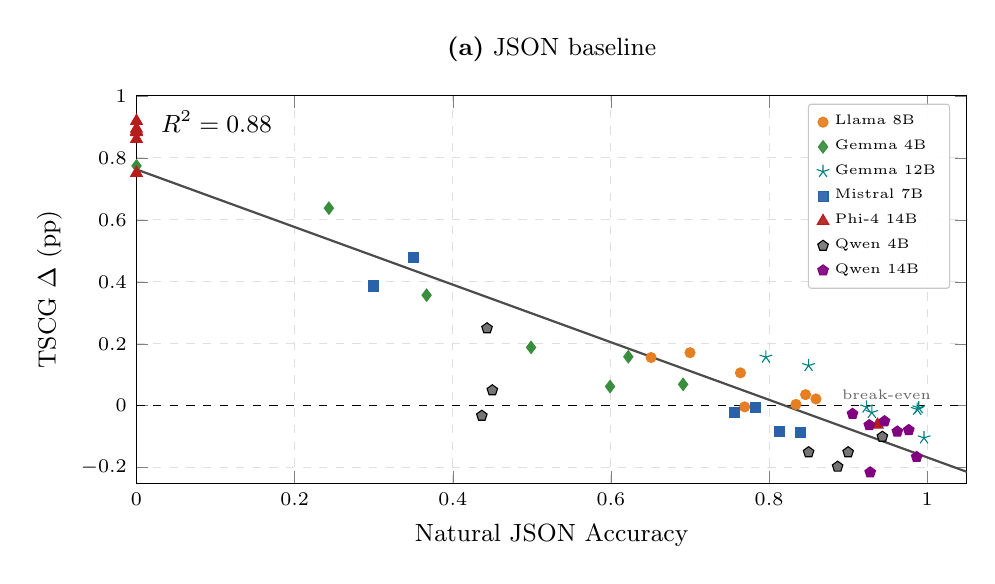
\begin{tikzpicture}
\begin{axis}[
    width=\textwidth,
    height=6.5cm,
    xlabel={Natural JSON Accuracy},
    ylabel={TSCG $\Delta$ (pp)},
    xlabel style={font=\small},
    ylabel style={font=\small},
    xmin=0, xmax=1.05,
    ymin=-0.25, ymax=1.0,
    xtick={0, 0.2, 0.4, 0.6, 0.8, 1.0},
    ytick={-0.2, 0, 0.2, 0.4, 0.6, 0.8, 1.0},
    tick label style={font=\scriptsize},
    grid=major,
    grid style={dashed, gray!25},
    clip=true,
    title={\textbf{(a)} JSON baseline},
    title style={font=\small, at={(0.5,1.02)}},
    legend style={
        at={(0.98,0.98)},
        anchor=north east,
        font=\tiny,
        draw=tscggray!40,
        fill=white,
        fill opacity=0.92,
        text opacity=1,
        rounded corners=1pt,
        row sep=0pt,
        /tikz/every even column/.append style={column sep=3pt},
    },
    legend cell align=left,
]

% ── Break-even line ──────────────────────────────────────────────────────────
\addplot[black, dashed, thin, forget plot] coordinates { (0, 0) (1.05, 0) };

% ── Regression: y = -0.9293x + 0.7626, R² = 0.88 ───────────────────────────
\addplot[black!70, thick, solid, forget plot, domain=0:1.05, samples=2]
    {-0.9293*x + 0.7626};

% ── Llama 3.1 8B (orange circles) ───────────────────────────────────────────
\addplot[only marks, mark=*, mark size=1.8pt, color=tscgorange, fill=tscgorange]
coordinates {
    (0.6508, 0.1557) (0.7000, 0.1713) (0.7691,-0.0036)
    (0.8462, 0.0359) (0.8340, 0.0044) (0.8593, 0.0220) (0.7638, 0.1062)
};
\addlegendentry{Llama 8B}

% ── Gemma 3 4B (green diamonds) ─────────────────────────────────────────────
\addplot[only marks, mark=diamond*, mark size=2.2pt, color=tscggreen, fill=tscggreen]
coordinates {
    (0.0000, 0.7743) (0.6220, 0.1580) (0.6913, 0.0691)
    (0.5989, 0.0620) (0.4990, 0.1883) (0.3669, 0.3569) (0.2433, 0.6378)
};
\addlegendentry{Gemma 4B}

% ── Gemma 3 12B (teal stars) ────────────────────────────────────────────────
\addplot[only marks, mark=star, mark size=2.4pt, color=tscgteal, fill=tscgteal]
coordinates {
    (0.9893,-0.0067) (0.9873,-0.0117) (0.9960,-0.1036)
    (0.9233,-0.0042) (0.7960, 0.1570) (0.9300,-0.0217) (0.8500, 0.1298)
};
\addlegendentry{Gemma 12B}

% ── Mistral 7B (blue squares) ───────────────────────────────────────────────
\addplot[only marks, mark=square*, mark size=1.8pt, color=tscgblue, fill=tscgblue]
coordinates {
    (0.7567,-0.0217) (0.7833,-0.0067) (0.8400,-0.0867)
    (0.8133,-0.0836) (0.3500, 0.4800) (0.3000, 0.3861) (0.3000, 0.3867)
};
\addlegendentry{Mistral 7B}

% ── Phi-4 14B (red triangles) ───────────────────────────────────────────────
\addplot[only marks, mark=triangle*, mark size=2.4pt, color=tscgred, fill=tscgred]
coordinates {
    (0.9371,-0.0617) (0.0000, 0.8827) (0.0000, 0.8940)
    (0.0000, 0.8868) (0.0000, 0.8611) (0.0000, 0.7513) (0.0000, 0.9190)
};
\addlegendentry{Phi-4 14B}

% ── Qwen3 4B (gray pentagons) ──────────────────────────────────────────────
\addplot[only marks, mark=pentagon*, mark size=2pt, color=black, fill=tscggray]
coordinates {
    (0.4367,-0.0322) (0.9433,-0.1000) (0.8867,-0.1967)
    (0.4500, 0.0500) (0.4433, 0.2500) (0.8500,-0.1500) (0.9000,-0.1500)
};
\addlegendentry{Qwen 4B}

% ── Qwen3 14B (purple pentagons) ───────────────────────────────────────────
\addplot[only marks, mark=pentagon*, mark size=2pt, color=tscgpurple, fill=tscgpurple]
coordinates {
    (0.9056,-0.0262) (0.9867,-0.1653) (0.9622,-0.0833)
    (0.9767,-0.0784) (0.9268,-0.0627) (0.9279,-0.2150) (0.9460,-0.0500)
};
\addlegendentry{Qwen 14B}

% ── R² annotation ───────────────────────────────────────────────────────────
\node[anchor=north west, font=\small\bfseries, fill=white, fill opacity=0.85,
    text opacity=1, inner sep=3pt, rounded corners=1pt]
    at (axis cs:0.02,0.98) {$R^2 = 0.88$};

\node[anchor=south west, font=\tiny, text=black!60]
    at (axis cs:0.88,-0.01) {break-even};

\end{axis}
\end{tikzpicture}
\end{subfigure}%
\hfill
\begin{subfigure}[t]{0.48\textwidth}
\centering
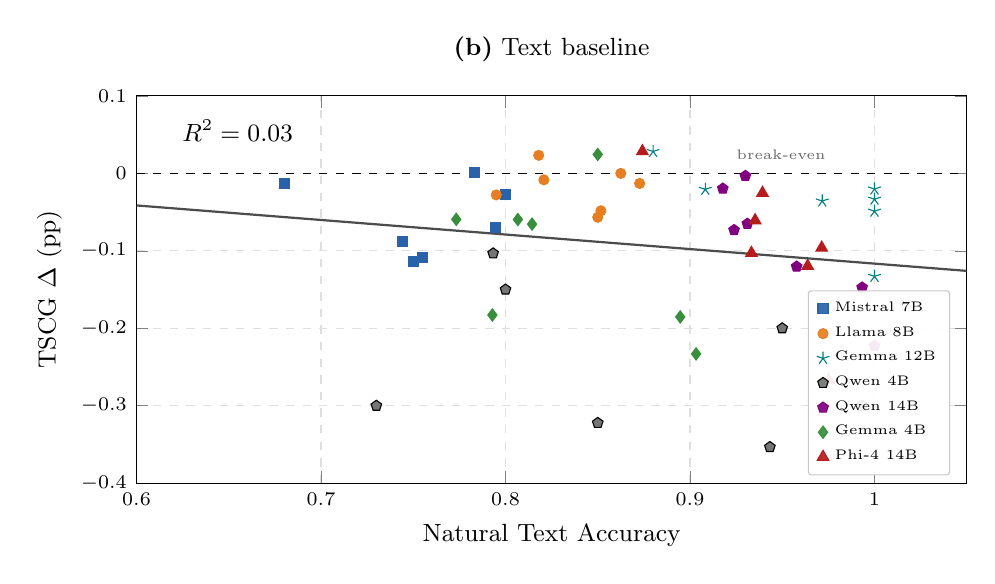
\begin{tikzpicture}
\begin{axis}[
    width=\textwidth,
    height=6.5cm,
    xlabel={Natural Text Accuracy},
    ylabel={TSCG $\Delta$ (pp)},
    xlabel style={font=\small},
    ylabel style={font=\small},
    xmin=0.6, xmax=1.05,
    ymin=-0.40, ymax=0.10,
    xtick={0.6, 0.7, 0.8, 0.9, 1.0},
    ytick={-0.4, -0.3, -0.2, -0.1, 0, 0.1},
    tick label style={font=\scriptsize},
    grid=major,
    grid style={dashed, gray!25},
    clip=true,
    title={\textbf{(b)} Text baseline},
    title style={font=\small, at={(0.5,1.02)}},
    legend style={
        at={(0.98,0.02)},
        anchor=south east,
        font=\tiny,
        draw=tscggray!40,
        fill=white,
        fill opacity=0.92,
        text opacity=1,
        rounded corners=1pt,
        row sep=0pt,
        /tikz/every even column/.append style={column sep=3pt},
    },
    legend cell align=left,
]

% ── Break-even line ──────────────────────────────────────────────────────────
\addplot[black, dashed, thin, forget plot] coordinates { (0.6, 0) (1.05, 0) };

% ── Regression: y = -0.1878x + 0.0713, R² = 0.03 ───────────────────────────
\addplot[black!70, thick, solid, forget plot, domain=0.6:1.05, samples=2]
    {-0.1878*x + 0.0713};

% ── Mistral 7B (blue squares) ───────────────────────────────────────────────
\addplot[only marks, mark=square*, mark size=1.8pt, color=tscgblue, fill=tscgblue]
coordinates {
    (0.7444,-0.0878) (0.8000,-0.0267) (0.7947,-0.0697)
    (0.6804,-0.0132) (0.7833, 0.0013) (0.7550,-0.1089) (0.7500,-0.1133)
};
\addlegendentry{Mistral 7B}

% ── Llama 3.1 8B (orange circles) ───────────────────────────────────────────
\addplot[only marks, mark=*, mark size=1.8pt, color=tscgorange, fill=tscgorange]
coordinates {
    (0.8500,-0.0567) (0.8517,-0.0483) (0.7950,-0.0278)
    (0.8208,-0.0083) (0.8727,-0.0130) (0.8180, 0.0233) (0.8625, 0.0000)
};
\addlegendentry{Llama 8B}

% ── Gemma 3 12B (teal stars) ────────────────────────────────────────────────
\addplot[only marks, mark=star, mark size=2.4pt, color=tscgteal, fill=tscgteal]
coordinates {
    (1.0000,-0.0333) (1.0000,-0.0488) (1.0000,-0.1329)
    (0.9083,-0.0206) (0.9717,-0.0357) (0.8800, 0.0283) (1.0000,-0.0202)
};
\addlegendentry{Gemma 12B}

% ── Qwen3 4B (gray pentagons) ──────────────────────────────────────────────
\addplot[only marks, mark=pentagon*, mark size=2pt, color=black, fill=tscggray]
coordinates {
    (0.7300,-0.3000) (0.9933,-0.3000) (0.7933,-0.1033)
    (0.8500,-0.3222) (0.9433,-0.3533) (0.8000,-0.1500) (0.9500,-0.2000)
};
\addlegendentry{Qwen 4B}

% ── Qwen3 14B (purple pentagons) ───────────────────────────────────────────
\addplot[only marks, mark=pentagon*, mark size=2pt, color=tscgpurple, fill=tscgpurple]
coordinates {
    (0.9578,-0.1203) (0.9300,-0.0033) (0.9311,-0.0650)
    (0.9239,-0.0731) (0.9178,-0.0196) (1.0000,-0.2227) (0.9933,-0.1473)
};
\addlegendentry{Qwen 14B}

% ── Gemma 3 4B (green diamonds) ─────────────────────────────────────────────
\addplot[only marks, mark=diamond*, mark size=2.2pt, color=tscggreen, fill=tscggreen]
coordinates {
    (0.8144,-0.0655) (0.8947,-0.1853) (0.8067,-0.0596)
    (0.7929,-0.1828) (0.9033,-0.2331) (0.7733,-0.0594) (0.8500, 0.0244)
};
\addlegendentry{Gemma 4B}

% ── Phi-4 14B (red triangles) ───────────────────────────────────────────────
\addplot[only marks, mark=triangle*, mark size=2.4pt, color=tscgred, fill=tscgred]
coordinates {
    (0.9714,-0.0960) (0.9353,-0.0607) (0.9393,-0.0253)
    (0.9333,-0.1029) (0.9638,-0.1196) (0.9750,-0.2670) (0.8742, 0.0285)
};
\addlegendentry{Phi-4 14B}

% ── R² annotation ───────────────────────────────────────────────────────────
\node[anchor=north west, font=\small\bfseries, fill=white, fill opacity=0.85,
    text opacity=1, inner sep=3pt, rounded corners=1pt]
    at (axis cs:0.62,0.08) {$R^2 = 0.03$};

\node[anchor=south west, font=\tiny, text=black!60]
    at (axis cs:0.92,0.005) {break-even};

\end{axis}
\end{tikzpicture}
\end{subfigure}
\caption{Format-confound decomposition of the predictive model. \textbf{(a)}~Against JSON baselines ($n{=}49$, 7 models $\times$ 7 catalog sizes), natural accuracy strongly predicts TSCG improvement ($R^2{=}0.88$, slope~${\approx}{-}0.93$): models that fail at JSON parsing gain the most. \textbf{(b)}~Against text baselines ($n{=}49$), the correlation vanishes ($R^2{=}0.03$, $p{=}0.24$): once the format confound is removed, baseline accuracy has no predictive power. The 97\% drop in $R^2$ confirms that the JSON-baseline regression captures format sensitivity, not compression benefit.}
\label{fig:natural-vs-delta}
\end{figure*}
 from main.tex
\begin{figure*}[t]
\centering
\begin{subfigure}[t]{0.48\textwidth}
\centering
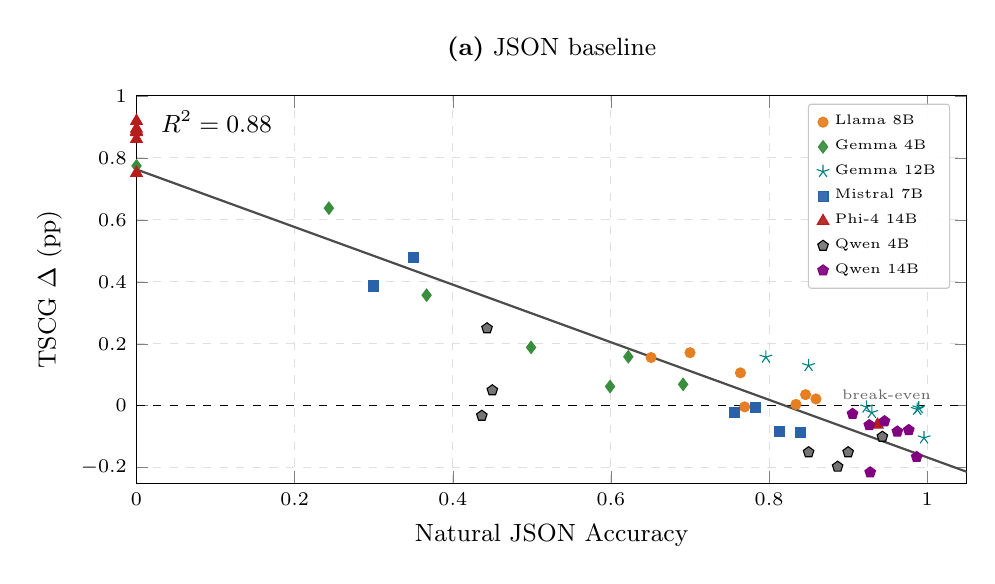
\begin{tikzpicture}
\begin{axis}[
    width=\textwidth,
    height=6.5cm,
    xlabel={Natural JSON Accuracy},
    ylabel={TSCG $\Delta$ (pp)},
    xlabel style={font=\small},
    ylabel style={font=\small},
    xmin=0, xmax=1.05,
    ymin=-0.25, ymax=1.0,
    xtick={0, 0.2, 0.4, 0.6, 0.8, 1.0},
    ytick={-0.2, 0, 0.2, 0.4, 0.6, 0.8, 1.0},
    tick label style={font=\scriptsize},
    grid=major,
    grid style={dashed, gray!25},
    clip=true,
    title={\textbf{(a)} JSON baseline},
    title style={font=\small, at={(0.5,1.02)}},
    legend style={
        at={(0.98,0.98)},
        anchor=north east,
        font=\tiny,
        draw=tscggray!40,
        fill=white,
        fill opacity=0.92,
        text opacity=1,
        rounded corners=1pt,
        row sep=0pt,
        /tikz/every even column/.append style={column sep=3pt},
    },
    legend cell align=left,
]

% ── Break-even line ──────────────────────────────────────────────────────────
\addplot[black, dashed, thin, forget plot] coordinates { (0, 0) (1.05, 0) };

% ── Regression: y = -0.9293x + 0.7626, R² = 0.88 ───────────────────────────
\addplot[black!70, thick, solid, forget plot, domain=0:1.05, samples=2]
    {-0.9293*x + 0.7626};

% ── Llama 3.1 8B (orange circles) ───────────────────────────────────────────
\addplot[only marks, mark=*, mark size=1.8pt, color=tscgorange, fill=tscgorange]
coordinates {
    (0.6508, 0.1557) (0.7000, 0.1713) (0.7691,-0.0036)
    (0.8462, 0.0359) (0.8340, 0.0044) (0.8593, 0.0220) (0.7638, 0.1062)
};
\addlegendentry{Llama 8B}

% ── Gemma 3 4B (green diamonds) ─────────────────────────────────────────────
\addplot[only marks, mark=diamond*, mark size=2.2pt, color=tscggreen, fill=tscggreen]
coordinates {
    (0.0000, 0.7743) (0.6220, 0.1580) (0.6913, 0.0691)
    (0.5989, 0.0620) (0.4990, 0.1883) (0.3669, 0.3569) (0.2433, 0.6378)
};
\addlegendentry{Gemma 4B}

% ── Gemma 3 12B (teal stars) ────────────────────────────────────────────────
\addplot[only marks, mark=star, mark size=2.4pt, color=tscgteal, fill=tscgteal]
coordinates {
    (0.9893,-0.0067) (0.9873,-0.0117) (0.9960,-0.1036)
    (0.9233,-0.0042) (0.7960, 0.1570) (0.9300,-0.0217) (0.8500, 0.1298)
};
\addlegendentry{Gemma 12B}

% ── Mistral 7B (blue squares) ───────────────────────────────────────────────
\addplot[only marks, mark=square*, mark size=1.8pt, color=tscgblue, fill=tscgblue]
coordinates {
    (0.7567,-0.0217) (0.7833,-0.0067) (0.8400,-0.0867)
    (0.8133,-0.0836) (0.3500, 0.4800) (0.3000, 0.3861) (0.3000, 0.3867)
};
\addlegendentry{Mistral 7B}

% ── Phi-4 14B (red triangles) ───────────────────────────────────────────────
\addplot[only marks, mark=triangle*, mark size=2.4pt, color=tscgred, fill=tscgred]
coordinates {
    (0.9371,-0.0617) (0.0000, 0.8827) (0.0000, 0.8940)
    (0.0000, 0.8868) (0.0000, 0.8611) (0.0000, 0.7513) (0.0000, 0.9190)
};
\addlegendentry{Phi-4 14B}

% ── Qwen3 4B (gray pentagons) ──────────────────────────────────────────────
\addplot[only marks, mark=pentagon*, mark size=2pt, color=black, fill=tscggray]
coordinates {
    (0.4367,-0.0322) (0.9433,-0.1000) (0.8867,-0.1967)
    (0.4500, 0.0500) (0.4433, 0.2500) (0.8500,-0.1500) (0.9000,-0.1500)
};
\addlegendentry{Qwen 4B}

% ── Qwen3 14B (purple pentagons) ───────────────────────────────────────────
\addplot[only marks, mark=pentagon*, mark size=2pt, color=tscgpurple, fill=tscgpurple]
coordinates {
    (0.9056,-0.0262) (0.9867,-0.1653) (0.9622,-0.0833)
    (0.9767,-0.0784) (0.9268,-0.0627) (0.9279,-0.2150) (0.9460,-0.0500)
};
\addlegendentry{Qwen 14B}

% ── R² annotation ───────────────────────────────────────────────────────────
\node[anchor=north west, font=\small\bfseries, fill=white, fill opacity=0.85,
    text opacity=1, inner sep=3pt, rounded corners=1pt]
    at (axis cs:0.02,0.98) {$R^2 = 0.88$};

\node[anchor=south west, font=\tiny, text=black!60]
    at (axis cs:0.88,-0.01) {break-even};

\end{axis}
\end{tikzpicture}
\end{subfigure}%
\hfill
\begin{subfigure}[t]{0.48\textwidth}
\centering
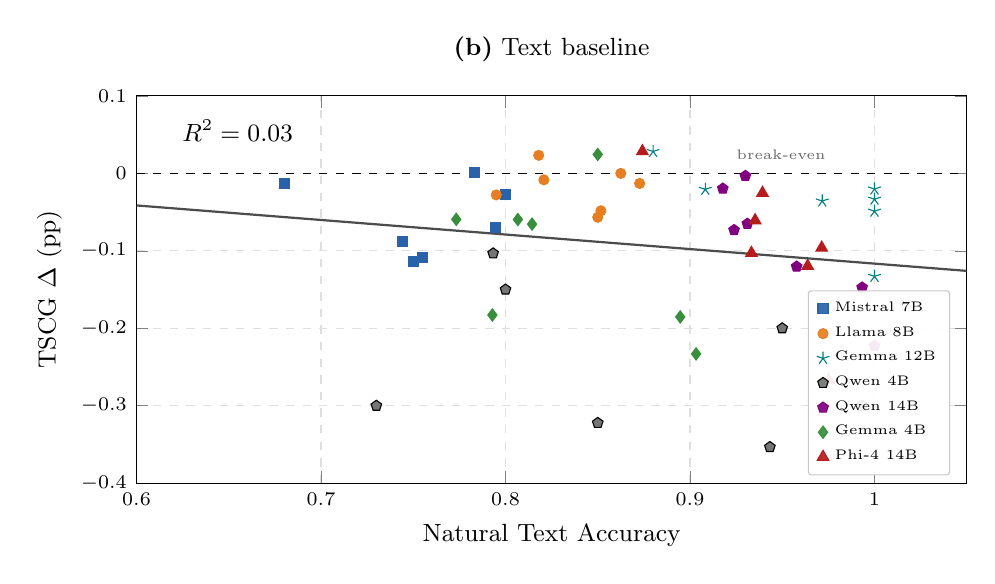
\begin{tikzpicture}
\begin{axis}[
    width=\textwidth,
    height=6.5cm,
    xlabel={Natural Text Accuracy},
    ylabel={TSCG $\Delta$ (pp)},
    xlabel style={font=\small},
    ylabel style={font=\small},
    xmin=0.6, xmax=1.05,
    ymin=-0.40, ymax=0.10,
    xtick={0.6, 0.7, 0.8, 0.9, 1.0},
    ytick={-0.4, -0.3, -0.2, -0.1, 0, 0.1},
    tick label style={font=\scriptsize},
    grid=major,
    grid style={dashed, gray!25},
    clip=true,
    title={\textbf{(b)} Text baseline},
    title style={font=\small, at={(0.5,1.02)}},
    legend style={
        at={(0.98,0.02)},
        anchor=south east,
        font=\tiny,
        draw=tscggray!40,
        fill=white,
        fill opacity=0.92,
        text opacity=1,
        rounded corners=1pt,
        row sep=0pt,
        /tikz/every even column/.append style={column sep=3pt},
    },
    legend cell align=left,
]

% ── Break-even line ──────────────────────────────────────────────────────────
\addplot[black, dashed, thin, forget plot] coordinates { (0.6, 0) (1.05, 0) };

% ── Regression: y = -0.1878x + 0.0713, R² = 0.03 ───────────────────────────
\addplot[black!70, thick, solid, forget plot, domain=0.6:1.05, samples=2]
    {-0.1878*x + 0.0713};

% ── Mistral 7B (blue squares) ───────────────────────────────────────────────
\addplot[only marks, mark=square*, mark size=1.8pt, color=tscgblue, fill=tscgblue]
coordinates {
    (0.7444,-0.0878) (0.8000,-0.0267) (0.7947,-0.0697)
    (0.6804,-0.0132) (0.7833, 0.0013) (0.7550,-0.1089) (0.7500,-0.1133)
};
\addlegendentry{Mistral 7B}

% ── Llama 3.1 8B (orange circles) ───────────────────────────────────────────
\addplot[only marks, mark=*, mark size=1.8pt, color=tscgorange, fill=tscgorange]
coordinates {
    (0.8500,-0.0567) (0.8517,-0.0483) (0.7950,-0.0278)
    (0.8208,-0.0083) (0.8727,-0.0130) (0.8180, 0.0233) (0.8625, 0.0000)
};
\addlegendentry{Llama 8B}

% ── Gemma 3 12B (teal stars) ────────────────────────────────────────────────
\addplot[only marks, mark=star, mark size=2.4pt, color=tscgteal, fill=tscgteal]
coordinates {
    (1.0000,-0.0333) (1.0000,-0.0488) (1.0000,-0.1329)
    (0.9083,-0.0206) (0.9717,-0.0357) (0.8800, 0.0283) (1.0000,-0.0202)
};
\addlegendentry{Gemma 12B}

% ── Qwen3 4B (gray pentagons) ──────────────────────────────────────────────
\addplot[only marks, mark=pentagon*, mark size=2pt, color=black, fill=tscggray]
coordinates {
    (0.7300,-0.3000) (0.9933,-0.3000) (0.7933,-0.1033)
    (0.8500,-0.3222) (0.9433,-0.3533) (0.8000,-0.1500) (0.9500,-0.2000)
};
\addlegendentry{Qwen 4B}

% ── Qwen3 14B (purple pentagons) ───────────────────────────────────────────
\addplot[only marks, mark=pentagon*, mark size=2pt, color=tscgpurple, fill=tscgpurple]
coordinates {
    (0.9578,-0.1203) (0.9300,-0.0033) (0.9311,-0.0650)
    (0.9239,-0.0731) (0.9178,-0.0196) (1.0000,-0.2227) (0.9933,-0.1473)
};
\addlegendentry{Qwen 14B}

% ── Gemma 3 4B (green diamonds) ─────────────────────────────────────────────
\addplot[only marks, mark=diamond*, mark size=2.2pt, color=tscggreen, fill=tscggreen]
coordinates {
    (0.8144,-0.0655) (0.8947,-0.1853) (0.8067,-0.0596)
    (0.7929,-0.1828) (0.9033,-0.2331) (0.7733,-0.0594) (0.8500, 0.0244)
};
\addlegendentry{Gemma 4B}

% ── Phi-4 14B (red triangles) ───────────────────────────────────────────────
\addplot[only marks, mark=triangle*, mark size=2.4pt, color=tscgred, fill=tscgred]
coordinates {
    (0.9714,-0.0960) (0.9353,-0.0607) (0.9393,-0.0253)
    (0.9333,-0.1029) (0.9638,-0.1196) (0.9750,-0.2670) (0.8742, 0.0285)
};
\addlegendentry{Phi-4 14B}

% ── R² annotation ───────────────────────────────────────────────────────────
\node[anchor=north west, font=\small\bfseries, fill=white, fill opacity=0.85,
    text opacity=1, inner sep=3pt, rounded corners=1pt]
    at (axis cs:0.62,0.08) {$R^2 = 0.03$};

\node[anchor=south west, font=\tiny, text=black!60]
    at (axis cs:0.92,0.005) {break-even};

\end{axis}
\end{tikzpicture}
\end{subfigure}
\caption{Format-confound decomposition of the predictive model. \textbf{(a)}~Against JSON baselines ($n{=}49$, 7 models $\times$ 7 catalog sizes), natural accuracy strongly predicts TSCG improvement ($R^2{=}0.88$, slope~${\approx}{-}0.93$): models that fail at JSON parsing gain the most. \textbf{(b)}~Against text baselines ($n{=}49$), the correlation vanishes ($R^2{=}0.03$, $p{=}0.24$): once the format confound is removed, baseline accuracy has no predictive power. The 97\% drop in $R^2$ confirms that the JSON-baseline regression captures format sensitivity, not compression benefit.}
\label{fig:natural-vs-delta}
\end{figure*}


\label{sec:naive-truncation}
At 16~tools, naive truncation matches TSCG (87.0\% vs.\ 87.8\%; Table~\ref{tab:naive-truncation}).
At 50~ambiguous tools, TSCG achieves 100\% vs.\ 98.5\%, with multi-tool sequencing driving the gap (87.5\% vs.\ 75.0\%).

\begin{table}[h]
\centering
\small
\caption{Naive truncation vs.\ TSCG (text-mode, Claude Sonnet~4).}
\label{tab:naive-truncation}
\begin{tabular}{llrrr}
\toprule
\textbf{Sc.} & \textbf{Condition} & \textbf{Savings} & \textbf{TSA} & \textbf{Overall} \\
\midrule
\multirow{3}{*}{A-16}
& Natural-Text     & ---    & 85.0 & 76.9 \\
& TSCG             & 17\% & 95.0 & 87.8 \\
& Naive trunc.     & 93\% & 95.0 & 87.0 \\
\midrule
\multirow{3}{*}{C-50}
& Natural-Text     & ---    & 95.0 & 95.0 \\
& TSCG             & 23\% & 100.0 & 100.0 \\
& Naive trunc.     & 87\% & 100.0 & 98.5 \\
\bottomrule
\end{tabular}
\end{table}

\subsection{External Validation}
\label{sec:bfcl-integration}

BFCL: 93.2\% on Berkeley Function Calling Leaderboard schemas (vs.\ 85.7\% natural; ARR~108\%, 46.8\% savings)---TSCG \emph{improves} accuracy on third-party benchmarks.
GSM8K-Under-Load: reasoning preserved (${\sim}$81\% across 0--50 tools); details in Appendix~\ref{app:gsm8k}.
Conservative SDM on Qwen3-14B: $+$4.4\,pp (balanced: $-$6.6\,pp); ablation in Appendix~\ref{app:sdm-detail} and Figure~\ref{fig:sdm-ablation}.

\begin{figure*}[t]
\centering
\begin{minipage}[t]{0.32\textwidth}
\centering
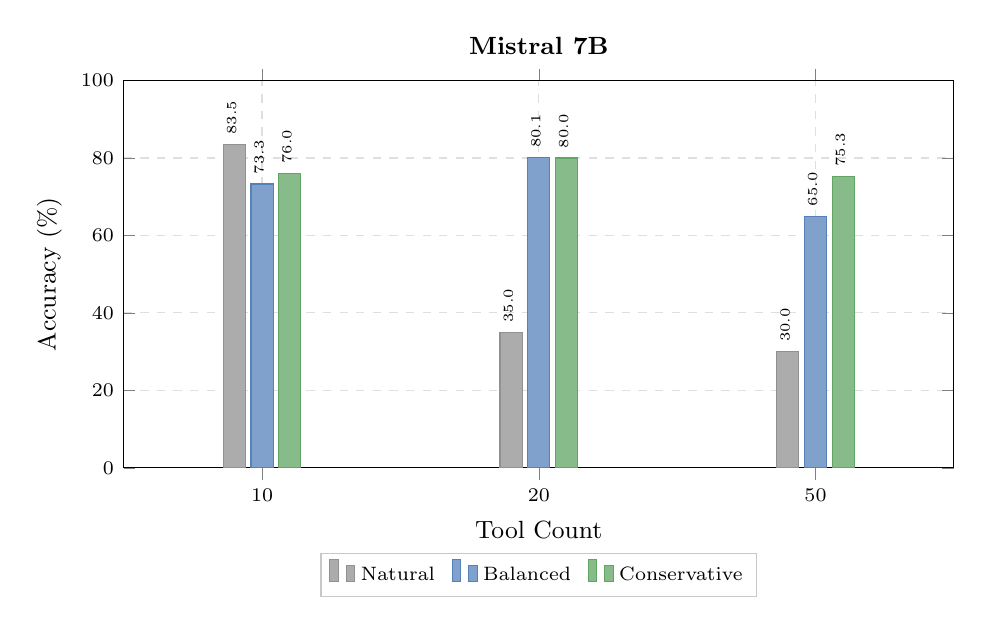
\begin{tikzpicture}
\begin{axis}[
    ybar,
    bar width=8pt,
    width=\textwidth,
    height=6.5cm,
    title={\small\textbf{Mistral 7B}},
    ylabel={Accuracy (\%)},
    ylabel style={font=\small},
    symbolic x coords={10, 20, 50},
    xtick=data,
    xlabel={Tool Count},
    xlabel style={font=\small},
    x tick label style={font=\scriptsize},
    ymin=0,
    ymax=100,
    ytick={0,20,40,60,80,100},
    y tick label style={font=\scriptsize},
    nodes near coords,
    nodes near coords style={font=\tiny, rotate=90, anchor=west},
    every node near coord/.append style={yshift=1pt},
    point meta=explicit symbolic,
    grid=major,
    grid style={dashed, gray!25},
    enlarge x limits=0.25,
    legend style={
        at={(0.5,-0.22)},
        anchor=north,
        legend columns=3,
        font=\scriptsize,
        /tikz/every even column/.append style={column sep=4pt},
        draw=tscggray!40,
    },
]

% Natural (gray)
\addplot[fill=tscggray!60, draw=tscggray!80] coordinates {
    (10, 83.5) [83.5]
    (20, 35.0) [35.0]
    (50, 30.0) [30.0]
};

% Balanced / TSCG (blue)
\addplot[fill=tscgblue!60, draw=tscgblue!80] coordinates {
    (10, 73.3) [73.3]
    (20, 80.1) [80.1]
    (50, 65.0) [65.0]
};

% Conservative (green)
\addplot[fill=tscggreen!60, draw=tscggreen!80] coordinates {
    (10, 76.0) [76.0]
    (20, 80.0) [80.0]
    (50, 75.3) [75.3]
};

\legend{Natural, Balanced, Conservative}

\end{axis}
\end{tikzpicture}
\end{minipage}%
\hfill
\begin{minipage}[t]{0.32\textwidth}
\centering
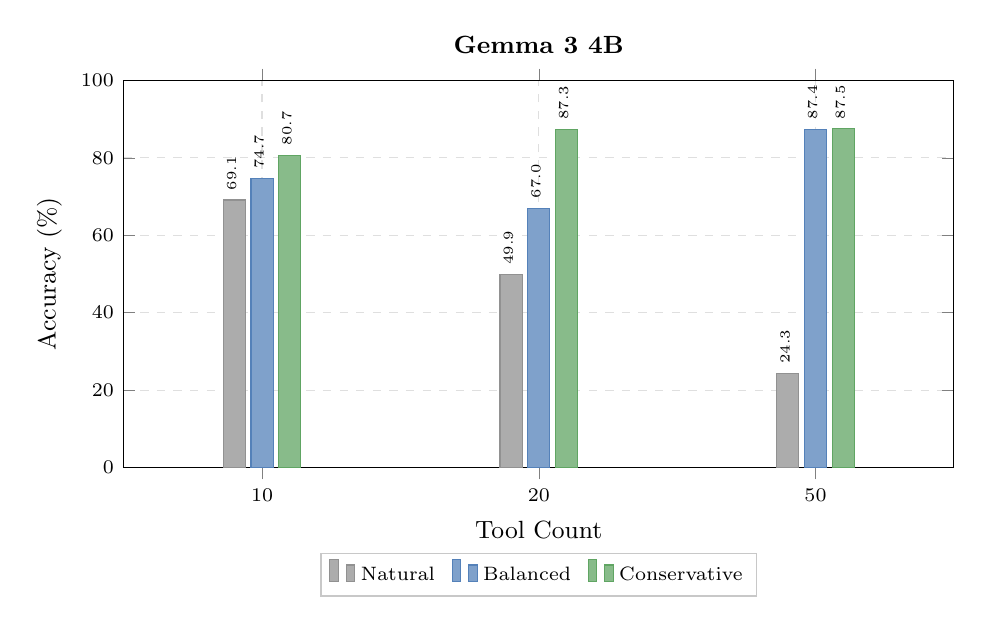
\begin{tikzpicture}
\begin{axis}[
    ybar,
    bar width=8pt,
    width=\textwidth,
    height=6.5cm,
    title={\small\textbf{Gemma 3 4B}},
    ylabel={Accuracy (\%)},
    ylabel style={font=\small},
    symbolic x coords={10, 20, 50},
    xtick=data,
    xlabel={Tool Count},
    xlabel style={font=\small},
    x tick label style={font=\scriptsize},
    ymin=0,
    ymax=100,
    ytick={0,20,40,60,80,100},
    y tick label style={font=\scriptsize},
    nodes near coords,
    nodes near coords style={font=\tiny, rotate=90, anchor=west},
    every node near coord/.append style={yshift=1pt},
    point meta=explicit symbolic,
    grid=major,
    grid style={dashed, gray!25},
    enlarge x limits=0.25,
    legend style={
        at={(0.5,-0.22)},
        anchor=north,
        legend columns=3,
        font=\scriptsize,
        /tikz/every even column/.append style={column sep=4pt},
        draw=tscggray!40,
    },
]

% Natural (gray)
\addplot[fill=tscggray!60, draw=tscggray!80] coordinates {
    (10, 69.1) [69.1]
    (20, 49.9) [49.9]
    (50, 24.3) [24.3]
};

% Balanced / TSCG (blue)
\addplot[fill=tscgblue!60, draw=tscgblue!80] coordinates {
    (10, 74.7) [74.7]
    (20, 67.0) [67.0]
    (50, 87.4) [87.4]
};

% Conservative (green)
\addplot[fill=tscggreen!60, draw=tscggreen!80] coordinates {
    (10, 80.7) [80.7]
    (20, 87.3) [87.3]
    (50, 87.5) [87.5]
};

\legend{Natural, Balanced, Conservative}

\end{axis}
\end{tikzpicture}
\end{minipage}%
\hfill
\begin{minipage}[t]{0.32\textwidth}
\centering
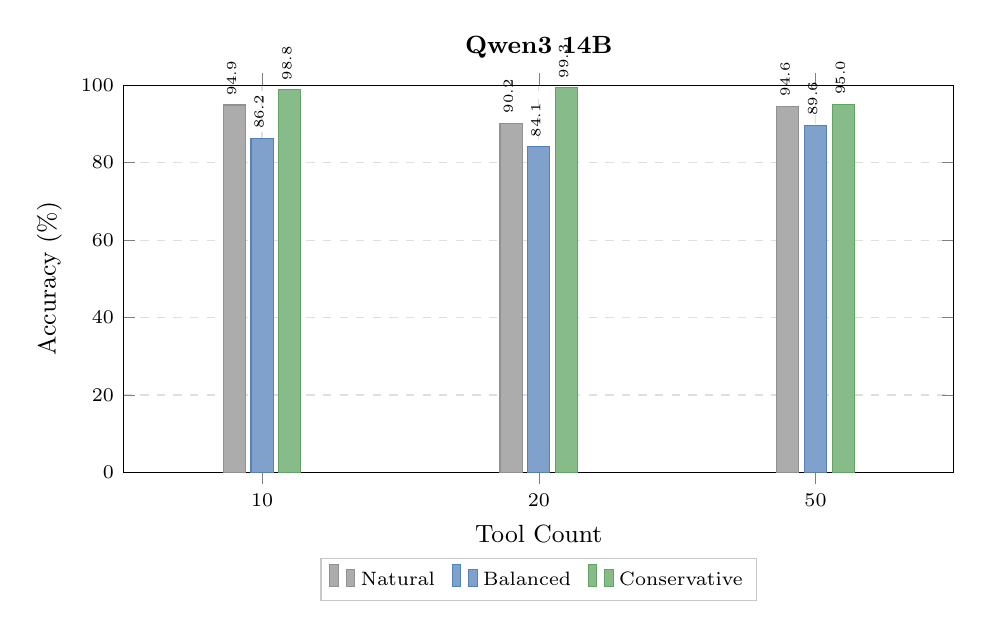
\begin{tikzpicture}
\begin{axis}[
    ybar,
    bar width=8pt,
    width=\textwidth,
    height=6.5cm,
    title={\small\textbf{Qwen3 14B}},
    ylabel={Accuracy (\%)},
    ylabel style={font=\small},
    symbolic x coords={10, 20, 50},
    xtick=data,
    xlabel={Tool Count},
    xlabel style={font=\small},
    x tick label style={font=\scriptsize},
    ymin=0,
    ymax=100,
    ytick={0,20,40,60,80,100},
    y tick label style={font=\scriptsize},
    nodes near coords,
    nodes near coords style={font=\tiny, rotate=90, anchor=west},
    every node near coord/.append style={yshift=1pt},
    point meta=explicit symbolic,
    grid=major,
    grid style={dashed, gray!25},
    enlarge x limits=0.25,
    legend style={
        at={(0.5,-0.22)},
        anchor=north,
        legend columns=3,
        font=\scriptsize,
        /tikz/every even column/.append style={column sep=4pt},
        draw=tscggray!40,
    },
]

% Natural (gray) — N3 re-run data (180 calls, profile bug corrected)
\addplot[fill=tscggray!60, draw=tscggray!80] coordinates {
    (10, 94.9) [94.9]
    (20, 90.2) [90.2]
    (50, 94.6) [94.6]
};

% Balanced / TSCG (blue)
\addplot[fill=tscgblue!60, draw=tscgblue!80] coordinates {
    (10, 86.2) [86.2]
    (20, 84.1) [84.1]
    (50, 89.6) [89.6]
};

% Conservative (green) — N3 re-run data (corrected: profile 'conservative' not 'minimal')
\addplot[fill=tscggreen!60, draw=tscggreen!80] coordinates {
    (10, 98.8) [98.8]
    (20, 99.3) [99.3]
    (50, 95.0) [95.0]
};

\legend{Natural, Balanced, Conservative}

\end{axis}
\end{tikzpicture}
\end{minipage}
\caption{SDM mode ablation across model sizes. \textbf{Left:} Mistral~7B ({<}10B). \textbf{Center:} Gemma~3~4B ({<}10B). \textbf{Right:} Qwen3~14B (14B, N3 re-run with corrected conservative profile). For small models (left, center), Conservative SDM matches or outperforms Balanced in 5 out of 6 conditions. For Qwen3~14B, Balanced TSCG degrades accuracy by {--}6.6\,pp mean, while Conservative mode \emph{improves} accuracy (mean~$\Delta$: {+}4.4\,pp), \emph{surpassing} Natural at 10 and 20~tools. Conservative SDM is universally safe and often beneficial.}
\label{fig:sdm-ablation}
\end{figure*}


% % Results section content merged into experiments.tex (TAB results).
% Pre-TAB results (19-task core benchmark, 11 runs, domain-specific,
% multi-model evaluation) relocated to Appendix~A.
  % Merged into experiments.tex; Pre-TAB → Appendix A
\section{Discussion}
\label{sec:discussion}

% Extended discussion content (CFL echo-back, rate-distortion analysis,
% LLMLingua comparison detail, NoTool bias, latency analysis, scope table,
% extended threats to validity, future directions) cut from main text.

\subsection{Three Mechanisms of TSCG Improvement}
\label{sec:three-mechanisms}

TSCG's accuracy improvements arise from three distinct mechanisms.
\textbf{M1: Format Translation} converts JSON schemas to structured text---the dominant mechanism for Class~1 models, where JSON parsing is the bottleneck (e.g., Phi-4: 0\%$\to$90\%, entirely format-driven per E1/E4).
\textbf{M2: Structural Reorganization} (CAS reordering, CFL constraint positioning, CFO causal ordering) improves accuracy beyond format change---the dominant mechanism for Class~2 frontier models ($+$10.9\,pp on Claude Sonnet~4 in text-mode, $+$24.4\,pp on GPT-5.2).
\textbf{M3: Token Reduction} decreases attention dilution as a secondary effect; GPT-4o achieves positive accuracy improvement even with negative token savings on certain scenarios, proving M2 operates independently of M3.

The mechanisms contribute differently per model class: M1 dominates for small models (Class~1), M2 for frontier models (Class~2), and neither contributes meaningfully for neutral models (Class~3). For Qwen architectures (Class~4), balanced M2 transforms actively harm accuracy, but conservative filler removal preserves benefits.

\subsection{Four-Class Taxonomy}
\label{sec:enabler-optimizer}

E4 text-baseline experiments (2{,}520 calls, 6~small models), N3 conservative ablation (180 calls), and N1 30B benchmarks (840 calls, 2~models) yield a four-class taxonomy across 12~models (Table~\ref{tab:four-class}):

\begin{table}[h]
\centering
\small
\caption{Four-class taxonomy of TSCG effects (12 models, 4B--32B + frontier). Text~$\Delta$: compression gain (TSCG minus text baseline).}
\label{tab:four-class}
\begin{tabular}{llrrl}
\toprule
\textbf{Class} & \textbf{Models} & \textbf{JSON $\Delta$} & \textbf{Text $\Delta$} & \textbf{Recommendation} \\
\midrule
1: Format-dom. & Phi-4, Mistral 7B, Gemma 4B, Qwen3 4B & +17 to +90\,pp & $-$7 to $-$23\,pp & Conservative \\
2: Compression & Claude, GPT-4o, GPT-5.2 & +5 to +11\,pp & +5 to +11\,pp & Balanced \\
3: Neutral & Llama 8B, Gemma 12B, Mistral-Sm.\ 24B & +5 to +9\,pp & $\approx$0\,pp & Conservative \\
4: Cons.-only & Qwen3 14B, Qwen2.5-Coder 32B & $-$5 to $-$7\,pp & $-$5 to $-$13\,pp & Conservative only \\
\bottomrule
\end{tabular}
\end{table}

\textbf{Class~1} models gain dramatically from JSON-baseline TSCG but show \emph{negative} compression against text baselines---the benefit is format translation (JSON$\to$text), confirmed by E4 decomposition.
\textbf{Class~2} frontier models show genuine structural compression ($+$5--11\,pp) that persists when format confound is eliminated.
\textbf{Class~3} models are robust across all formats; TSCG neither helps nor harms.
\textbf{Class~4} Qwen models degrade under balanced TSCG but improve $+$4.4\,pp under conservative SDM (N3)---the degradation is architecture-specific, persisting from 14B to 32B (N1), implicating CAS/DRO structural transforms rather than capacity limitations.

\paragraph{Deployment guidance.} Since every production API transmits JSON: (1)~Class~1 models achieve 0--49\% at $>$15 tools but 65--90\% under TSCG---format translation is the needed intervention; (2)~Class~2 benefits from balanced profiles; (3)~Class~4 requires conservative mode exclusively; (4)~Class~3 can use TSCG without risk.

\subsection{Naive Truncation Honesty}
\label{sec:naive-truncation-discussion}

At 16~well-named tools (Scenario~A), naive truncation (retaining only \texttt{ToolName(param:type,...)}) matches TSCG: 87.0\% vs.\ 87.8\% overall.
Claude Sonnet~4 recognizes tools by distinctive names, making descriptions dispensable.
The gap emerges at scale: at 50~tools with ambiguous names (Scenario~C-50), TSCG achieves 100\% while naive truncation drops to 98.5\%, concentrated in multi-tool sequencing (87.5\% vs.\ 75.0\%, $-$12.5\,pp) and parameter extraction (100\% vs.\ 92.5\%).
TSCG's structural reorganization preserves the semantic cues needed for disambiguation---parameter descriptions, usage constraints, return types---that naive truncation discards.

\subsection{Infrastructure Impact}
\label{sec:infrastructure-discussion}

TSCG reduces per-call schema overhead from $O(n \cdot k)$ to $O(n \cdot k/c)$ where $c \approx 3.5\times$ for structured schemas.
At production volumes (100k calls/day with 16~tools at \$3/MTok), the savings exceed \$30{,}000/month.
Combined with sub-millisecond deterministic execution, zero dependencies, and a 27.7\,KB bundle, TSCG deploys as transparent middleware in any agent framework---Claude Code, LangChain, CrewAI, or MCP servers---without GPU infrastructure or external API calls.

For small models (4B--14B), the infrastructure impact extends beyond cost: TSCG enables deployment of local models as functional tool-use agents in edge, cost-sensitive, and privacy-constrained environments where frontier APIs are unavailable or unacceptable.

\section{Limitations}
\label{sec:limitations}

% Extended threats to validity cut from main text.

\textbf{Benchmark scope.} TAB is self-constructed; we mitigate this with BFCL external validation (ARR 108\%), but independent third-party evaluation on diverse tool catalogs is needed.

\textbf{Task coverage.} TAB measures tool selection accuracy and parameter extraction only---not generation quality, multi-turn coherence, or end-to-end task completion.

\textbf{Small-model degradation.} Class~1 models show negative compression gains against text baselines ($-$7 to $-$23\,pp), meaning TSCG actively harms accuracy in hypothetical text-mode deployments with $<$10 tools.

\textbf{Language.} The filler pattern library and all evaluations are English-only. BPE tokenizations and filler patterns differ across languages; multilingual extension requires language-specific libraries.

\textbf{Model coverage.} 12 models tested across 4 architecture families. Generalization to untested architectures (e.g., Mamba, RWKV) is uncertain. Thinking models (o1, o3-mini, Gemini 2.5 Pro) are excluded---they produce empty responses on TSCG-compressed prompts.

\textbf{Predictive model precision.} LOO RMSE of 12.8\,pp provides coarse triage only; Phi-4's zero-accuracy leverage points inflate $R^2$ (excluding Phi-4: $R^2{=}0.81$).

\section{Conclusion}
\label{sec:conclusion}

We have presented Token-Context Semantic Grammar (TSCG), a deterministic tool-schema compiler that addresses the dominant token cost in agentic AI deployments.

\textbf{JSON-API enablement.} Every production framework transmits tools as JSON, yet small models (4B--14B) achieve only 0--49\% accuracy at $>$15 JSON-format tools.
TSCG recovers accuracy to 65--90\% by implicitly translating JSON schemas to structured text---enabling small models as functional tool-use agents in edge, cost-sensitive, and privacy-constrained environments.
E1/E4 (2{,}940 Ollama calls across 6 models) identifies format translation as the dominant mechanism for this class.

\textbf{Frontier compression.} For frontier models (Claude Sonnet~4, GPT-4o, GPT-5.2), TSCG provides genuine structural compression ($+$5--11\,pp, 50--72\% token savings) that persists when the format confound is eliminated.
At production volumes, this exceeds \$30{,}000/month in savings.

\textbf{Mechanistic decomposition.} The first format-vs-compression analysis for tool-schema optimization yields a four-class taxonomy across 12 models (4B--32B + frontier), with actionable deployment guidance: conservative SDM for small and Qwen models, balanced for frontier.
The predictive model ($R^2{=}0.88$, collapsing to 0.03 against text baselines) quantifies format sensitivity and enables deployment triage from a single baseline measurement.

TSCG is released as an open-source npm package---1{,}200 LOC TypeScript, zero dependencies, sub-millisecond execution, 27.7\,KB bundle.\footnote{\url{https://github.com/SKZL-AI/tscg}}
TAB, the first tool-schema compression benchmark (\tscgTotalCalls{} calls, 12 models, 5 scenarios), and all evaluation code are released as open-source infrastructure for the agent framework stack.

% % Implementation and Deployment section relocated to Appendix~F.
% Key implementation facts retained in Conclusion:
% @tscg/core, 1,200 LOC TypeScript, zero dependencies,
% sub-millisecond execution, 27.7 KB bundle.
  % Relocated to Appendix F

\bibliographystyle{acl_natbib}
\bibliography{references}

\appendix

% ============================================================================
% Appendix A: Pre-TAB Evaluation
% ============================================================================
\section{Pre-TAB Evaluation}
\label{app:pre-tab}

The pre-TAB evaluation comprised 19 core tasks across 7 categories (Factual $n{=}4$, Reasoning $n{=}4$, Classification $n{=}2$, Extraction $n{=}1$, OptFirst $n{=}3$, Complex $n{=}2$, NearDup $n{=}3$), 6 compression strategies, 11 independent runs on Claude Sonnet~4, and domain-specific benchmarks across 4 phases. This evaluation established TSCG's baseline effectiveness before the multi-model TAB benchmark. Full results are available in the supplementary materials.

% ============================================================================
% Appendix B: GSM8K-Under-Load
% ============================================================================
\section{GSM8K-Under-Load}
\label{app:gsm8k}

Tool-schema overhead does not degrade reasoning: Claude Sonnet~4 maintains ${\sim}$81\% GSM8K accuracy across 0--50 irrelevant tool definitions (${\sim}$400 calls). TSCG provides a consistent ${\sim}$4.5\,pp advantage over natural schemas, suggesting that reduced schema overhead frees attention capacity for mathematical reasoning. The effect is statistically significant ($+$4.5\,pp, $p = 0.020$) but practically small (Cohen's $d = 0.11$).

% ============================================================================
% Appendix C: SDM Ablation Detail
% ============================================================================
\section{SDM Ablation Detail}
\label{app:sdm-detail}

Conservative SDM (filler removal only) is compared with Balanced (full structural compression) on Qwen3-14B (180~calls, N3 corrected re-run at sizes 10/20/50):

\begin{itemize}[noitemsep]
    \item Balanced TSCG degrades accuracy by $-$6.6\,pp mean (90.2\%$\to$84.1\% at 20 tools, 94.6\%$\to$89.6\% at 50 tools).
    \item Conservative SDM \emph{improves} accuracy by $+$4.4\,pp mean (90.2\%$\to$99.3\% at 20 tools, 94.6\%$\to$95.0\% at 50 tools).
    \item CAS reordering and bracket elision---not SDM filler removal---trigger the degradation.
\end{itemize}

\noindent Practical recommendation: Conservative SDM for all models ${<}$10B and all Qwen architectures (including Qwen2.5-Coder~32B, confirmed by N1); Balanced for frontier models where genuine compression persists.

% ============================================================================
% Appendix D: Predictive Model + LOO + R² Robustness
% ============================================================================
\section{Predictive Model and LOO Cross-Validation}
\label{app:loo-details}

Table~\ref{tab:r2-robustness} reports robustness checks on the predictive regression (Equation~\ref{eq:correlation}).

\begin{table}[h]
\centering
\small
\caption{R\textsuperscript{2} robustness checks for the accuracy-gap regression.}
\label{tab:r2-robustness}
\begin{tabular}{@{}lcccc@{}}
\toprule
\textbf{Configuration} & $n$ & $R^2$ & \textbf{95\% CI} & $p$ \\
\midrule
7-model full set & 49 & 0.885 & $[0.78,\; 0.93]$ & $< 10^{-20}$ \\
7-model sans Phi-4 & 42 & 0.813 & $[0.58,\; 0.94]$ & $< 10^{-10}$ \\
Model-level (7 means) & 7 & 0.951 & $[0.62,\; 1.00]$ & $< 0.001$ \\
Text baseline (E4) & 49 & 0.028 & --- & 0.24 \\
\bottomrule
\end{tabular}
\end{table}

\noindent Phi-4~14B is the strongest leverage point ($\Delta R^2 = -0.07$ when removed), but $R^2$ remains above 0.80 without it. The linear relationship holds at the model level ($R^2 = 0.95$). LOO cross-validation (holding out one model, refitting on remaining six) yields RMSE~=~12.8\,pp---adequate for deployment triage but insufficient for precise predictions. Qwen3~4B is the only model where the prediction direction is wrong (predicted positive, actual negative), reflecting its volatile behavior.

% ============================================================================
% Appendix E: Theorem Proofs
% ============================================================================
\section{Theorem Proofs}
\label{app:proofs}

\begin{proof}[Proof of Theorem~\ref{thm:compression}]
Each token-reducing operator $T_i \in \mathcal{T}_R$ acts on a disjoint subset of tokens:
\begin{itemize}[noitemsep]
    \item \textbf{SDM}: filler patterns (104+ curated, non-overlapping with delimiters/tokenizer targets).
    \item \textbf{DRO}: verbose delimiter phrases (structural role markers).
    \item \textbf{TAS}: suboptimal tokenizer splits (multi-token $\to$ single-token Unicode).
    \item \textbf{CFL}: positional relocation of output constraint to position~0.
\end{itemize}
Disjoint action $\implies$ additive composition. $\mathcal{T}_S$ preserves count; $B{=}0$ excludes expansion:
\[
    |\tok(\Pi(S))| \;\leq\; |\tok(S)| \cdot \Bigl(1 - \sum_{T_i \in \mathcal{T}_R} r_i \cdot f_i(S)\Bigr). \qedhere
\]
\end{proof}

% ============================================================================
% Appendix F: Implementation Details
% ============================================================================
\section{Implementation and Deployment}
\label{app:deployment}

TSCG is implemented as ${\sim}$1{,}200 lines of TypeScript with zero external dependencies. Three deployment modes: CLI (npm), Chrome Extension (Manifest~V3), and Web Application (React + Vite). Production bundle: 27.7\,KB (10\,KB gzipped). Sub-millisecond execution for prompts under 4{,}096 tokens. Five optimization profiles (Table~\ref{tab:profiles}):

\begin{table}[h]
\centering
\small
\caption{TSCG optimization profiles.}
\label{tab:profiles}
\begin{tabular}{@{}lp{5cm}@{}}
\toprule
\textbf{Profile} & \textbf{Active Principles} \\
\midrule
\texttt{minimal} & SDM, CFL \\
\texttt{balanced} & SDM, DRO, CFL, CFO, TAS \\
\texttt{max\_compress} & SDM, DRO, CFL, CFO, TAS \\
\texttt{max\_accuracy} & SDM, CFL, DRO, TAS, CCP, SAD-F \\
\texttt{full} & All 8 principles \\
\bottomrule
\end{tabular}
\end{table}

% ============================================================================
% Appendix G: 21-System Prior-Art Table
% ============================================================================
\section{Extended Prior-Art Comparison}
\label{app:prior-art}

\begin{table*}[t]
\centering
\small
\setlength{\tabcolsep}{3.5pt}
\begin{tabular}{@{}l c c c c c c c c@{}}
\toprule
\textbf{System} & \textbf{Determ.} & \textbf{Tok-Aware} & \textbf{Causal Th.} & \textbf{Black-Box} & \textbf{Budg. Anch.} & \textbf{Compress.} & \textbf{No Train} & \textbf{Zero-Dep} \\
\midrule
\multicolumn{9}{l}{\textit{Compression-Based}} \\
\cmidrule(r){1-1}
LLMLingua \cite{jiang2023llmlingua}         & \xmark & \xmark & \xmark & \cmark & \cmark & \cmark & \xmark & \xmark \\
LLMLingua-2 \cite{pan2024llmlingua2}        & \xmark & \xmark & \xmark & \cmark & \cmark & \cmark & \xmark & \xmark \\
Selective Context \cite{li2023compressing}   & \cmark & \xmark & \xmark & \cmark & \xmark & \cmark & \cmark & \xmark \\
LongLLMLingua \cite{jiang2024longllmlingua}  & \xmark & \xmark & \xmark & \cmark & \cmark & \cmark & \xmark & \xmark \\
Gist Tokens \cite{mu2023learning}            & \xmark & \xmark & \xmark & \xmark & \xmark & \cmark & \xmark & \xmark \\
AutoCompressors \cite{chevalier2023adapting} & \xmark & \xmark & \xmark & \xmark & \xmark & \cmark & \xmark & \xmark \\
LeanContext \cite{arefeen2024leancontext}    & \xmark & \xmark & \xmark & \cmark & \xmark & \cmark & \xmark & \xmark \\
\midrule
\multicolumn{9}{l}{\textit{Search-Based}} \\
\cmidrule(r){1-1}
DSPy \cite{khattab2023dspy}                  & \xmark & \xmark & \xmark & \cmark & \xmark & \xmark & \cmark & \xmark \\
OPRO \cite{yang2024large}                    & \xmark & \xmark & \xmark & \cmark & \xmark & \xmark & \cmark & \xmark \\
APE \cite{zhou2023large}                     & \xmark & \xmark & \xmark & \cmark & \xmark & \xmark & \cmark & \xmark \\
EvoPrompt \cite{chen2024evoprompt}           & \xmark & \xmark & \xmark & \cmark & \xmark & \xmark & \cmark & \xmark \\
PromptBreeder \cite{fernando2024promptbreeder} & \xmark & \xmark & \xmark & \cmark & \xmark & \xmark & \cmark & \xmark \\
COSP \cite{wan2024cosp}                      & \xmark & \xmark & \xmark & \cmark & \xmark & \xmark & \cmark & \xmark \\
\midrule
\multicolumn{9}{l}{\textit{Gradient-Based}} \\
\cmidrule(r){1-1}
TextGrad \cite{yuksekgonul2024textgrad}      & \xmark & \xmark & \xmark & \xmark & \xmark & \xmark & \cmark & \xmark \\
ProTeGi \cite{pryzant2023automatically}      & \xmark & \xmark & \xmark & \xmark & \xmark & \xmark & \cmark & \xmark \\
PromptAgent \cite{wang2023promptagent}       & \xmark & \xmark & \xmark & \cmark & \xmark & \xmark & \cmark & \xmark \\
\midrule
\multicolumn{9}{l}{\textit{Template / Theoretical}} \\
\cmidrule(r){1-1}
LangGPT \cite{wang2024langgpt}              & \cmark & \xmark & \xmark & \cmark & \xmark & \xmark & \cmark & \xmark \\
SSR++ \cite{wen2024ssr}                      & \cmark & \xmark & \xmark & \cmark & \xmark & \xmark & \cmark & \xmark \\
CFPO \cite{guo2024cfpo}                      & \xmark & \xmark & \cmark & \cmark & \xmark & \xmark & \cmark & \xmark \\
\midrule
\textbf{TSCG (ours)}                         & \cmark & \cmark & \cmark & \cmark & \cmark & \cmark & \cmark & \cmark \\
\bottomrule
\end{tabular}
\caption{Comparison of 18 prompt optimization systems and TSCG across eight desiderata. \textbf{Determ.}: deterministic output for the same input. \textbf{Tok-Aware}: optimizes with respect to BPE tokenizer boundaries. \textbf{Causal Th.}: grounded in causal attention theory. \textbf{Black-Box}: requires no access to model weights or gradients. \textbf{Budg. Anch.}: budget-constrained anchor duplication. \textbf{Compress.}: achieves measurable token compression. \textbf{No Train}: requires no model training or fine-tuning. \textbf{Zero-Dep}: zero external runtime dependencies. TSCG is the only system satisfying all eight criteria.}
\label{tab:prior-art}
\end{table*}


% ============================================================================
% Appendix H: Benchmark Configurations + Statistical Detail
% ============================================================================
\section{Benchmark Configurations and Statistical Detail}
\label{app:configs}

Table~\ref{tab:run-configs} documents configuration parameters for all benchmark runs.

\begin{table}[h]
\centering
\small
\caption{Experimental configurations.}
\label{tab:run-configs}
\begin{tabular}{@{}llll@{}}
\toprule
\textbf{Parameter} & \textbf{Core/Domain} & \textbf{TAB} & \textbf{Ollama} \\
\midrule
Temperature & 0 & 0 & 0 \\
Seed & N/A & 42 & 42 \\
Max tokens & 4096 & 1024 & 1024 \\
Mode & Text + FC & Text-mode & Text-mode \\
SDM profile & full & balanced & balanced \\
API provider & Anthropic/OpenAI & Anthropic & Ollama (local) \\
Eval. method & Automated & TABEvaluator & TABEvaluator \\
\bottomrule
\end{tabular}
\end{table}

\subsection{Holm-Bonferroni Correction}
\label{app:holm-bonferroni}

107 pairwise McNemar tests, family-wise $\alpha = 0.05$. 9/107 achieve significance (Table~\ref{tab:holm-bonferroni}), all from Scenario~D with weak JSON baselines.

\begin{table}[h]
\centering
\small
\caption{Significant comparisons after Holm-Bonferroni ($\alpha = 0.05$, 107 tests).}
\label{tab:holm-bonferroni}
\begin{tabular}{@{}llcrr@{}}
\toprule
\textbf{Model} & \textbf{Tools} & \textbf{$\Delta$pp} & \textbf{$p_{\mathrm{adj}}$} & \textbf{$d$} \\
\midrule
Phi-4 14B    & 5/10/15 & $+$95.0 & 0.003 & 6.11 \\
Phi-4 14B    & 20 & $+$84.4 & 0.003 & 4.21 \\
Phi-4 14B    & 30 & $+$80.0 & 0.011 & 2.81 \\
Phi-4 14B    & 50 & $+$90.3 & 0.003 & 6.11 \\
Gemma 3 4B   & 3  & $+$85.0 & 0.007 & 3.34 \\
Gemma 3 4B   & 50 & $+$63.1 & 0.004 & 1.68 \\
Gemma 3 4B   & 50\textsuperscript{c} & $+$65.0 & 0.004 & 1.73 \\
\bottomrule
\end{tabular}
\end{table}

\subsection{Bootstrap Confidence Intervals}
\label{app:bootstrap-ci}

\begin{table}[h]
\centering
\small
\caption{Bootstrap 95\% CIs for key deltas (1{,}000 resamples, seed=42).}
\label{tab:bootstrap-ci}
\begin{tabular}{@{}llrrl@{}}
\toprule
\textbf{Scenario} & \textbf{Model} & \textbf{$\Delta$pp} & \textbf{95\% CI} & \textbf{$p$} \\
\midrule
A (16 tools) & Claude Sonnet 4 & $+$10.0 & [0.6, 18.3] & 0.200 \\
A (16 tools) & GPT-5.2 & $+$29.7 & [16.1, 42.2] & 0.004 \\
B (43 tools) & Claude Sonnet 4 & $+$5.3 & [$-$0.3, 11.3] & 0.063 \\
D (50 tools) & Phi-4 14B & $+$90.3 & --- & $<$0.001 \\
D (50 tools) & Gemma 3 4B & $+$63.1 & [45.0, 80.0] & $<$0.001 \\
GSM8K (50)   & Claude Sonnet 4 & $+$4.5 & [0.5, 8.5] & 0.020 \\
\bottomrule
\end{tabular}
\end{table}

\end{document}
